\documentclass[a4paper]{book}
\usepackage{a4wide}
\usepackage{makeidx}
\usepackage{graphicx}
\usepackage{multicol}
\usepackage{float}
\usepackage{listings}
\usepackage{color}
\usepackage{textcomp}
\usepackage{alltt}
\usepackage{times}
\usepackage{ifpdf}
\ifpdf
\usepackage[pdftex,
            pagebackref=true,
            colorlinks=true,
            linkcolor=blue,
            unicode
           ]{hyperref}
\else
\usepackage[ps2pdf,
            pagebackref=true,
            colorlinks=true,
            linkcolor=blue,
            unicode
           ]{hyperref}
\usepackage{pspicture}
\fi
\usepackage[utf8]{inputenc}
\usepackage{doxygen}
\lstset{language=C++,inputencoding=utf8,basicstyle=\footnotesize,breaklines=true,breakatwhitespace=true,tabsize=8,numbers=left }
\makeindex
\setcounter{tocdepth}{3}
\renewcommand{\footrulewidth}{0.4pt}
\begin{document}
\hypersetup{pageanchor=false}
\begin{titlepage}
\vspace*{7cm}
\begin{center}
{\Large ComboTabBar }\\
\vspace*{1cm}
{\large Generated by Doxygen 1.6.3}\\
\vspace*{0.5cm}
{\small Fri May 23 02:37:38 2014}\\
\end{center}
\end{titlepage}
\clearemptydoublepage
\pagenumbering{roman}
\tableofcontents
\clearemptydoublepage
\pagenumbering{arabic}
\hypersetup{pageanchor=true}
\chapter{Main Page}
\label{index}\hypertarget{index}{}It's a scrollable tabbar with pinned tab feature, its API is mostly similar to QTabBar's API. \begin{DoxyAuthor}{Author}
\href{https://github.com/srazi}{\tt Razi Alavizadeh} 

\href{https://github.com/nowrep}{\tt David Rosca} 
\end{DoxyAuthor}
\begin{DoxyDate}{Date}
2013-\/2014
\end{DoxyDate}
{\bfseries Main Class:} \hyperlink{class_combo_tab_bar}{ComboTabBar} 
\chapter{Class Index}
\section{Class Hierarchy}
This inheritance list is sorted roughly, but not completely, alphabetically:\begin{DoxyCompactList}
\item \contentsline{section}{QAbstractButton}{\pageref{class_q_abstract_button}}{}
\begin{DoxyCompactList}
\item \contentsline{section}{CloseButton}{\pageref{class_close_button}}{}
\end{DoxyCompactList}
\item \contentsline{section}{QScrollBar}{\pageref{class_q_scroll_bar}}{}
\begin{DoxyCompactList}
\item \contentsline{section}{TabScrollBar}{\pageref{class_tab_scroll_bar}}{}
\end{DoxyCompactList}
\item \contentsline{section}{QTabBar}{\pageref{class_q_tab_bar}}{}
\begin{DoxyCompactList}
\item \contentsline{section}{TabBarHelper}{\pageref{class_tab_bar_helper}}{}
\end{DoxyCompactList}
\item \contentsline{section}{QWidget}{\pageref{class_q_widget}}{}
\begin{DoxyCompactList}
\item \contentsline{section}{ComboTabBar}{\pageref{class_combo_tab_bar}}{}
\item \contentsline{section}{TabBarScrollWidget}{\pageref{class_tab_bar_scroll_widget}}{}
\item \contentsline{section}{TabStackedWidget}{\pageref{class_tab_stacked_widget}}{}
\end{DoxyCompactList}
\end{DoxyCompactList}

\chapter{Class Index}
\section{Class List}
Here are the classes, structs, unions and interfaces with brief descriptions:\begin{DoxyCompactList}
\item\contentsline{section}{\hyperlink{class_close_button}{CloseButton} (Class for close button on tabs $\ast$ taken from qtabbar.cpp )}{\pageref{class_close_button}}{}
\item\contentsline{section}{\hyperlink{class_combo_tab_bar}{ComboTabBar} (Mixed of a pinned tabbar and a normal scrollable tabbar )}{\pageref{class_combo_tab_bar}}{}
\item\contentsline{section}{\hyperlink{class_q_abstract_button}{QAbstractButton} }{\pageref{class_q_abstract_button}}{}
\item\contentsline{section}{\hyperlink{class_q_scroll_bar}{QScrollBar} }{\pageref{class_q_scroll_bar}}{}
\item\contentsline{section}{\hyperlink{class_q_tab_bar}{QTabBar} }{\pageref{class_q_tab_bar}}{}
\item\contentsline{section}{\hyperlink{class_q_widget}{QWidget} }{\pageref{class_q_widget}}{}
\item\contentsline{section}{\hyperlink{class_tab_bar_helper}{TabBarHelper} (A subclass of \hyperlink{class_q_tab_bar}{QTabBar} that can be inactivated )}{\pageref{class_tab_bar_helper}}{}
\item\contentsline{section}{\hyperlink{class_tab_bar_scroll_widget}{TabBarScrollWidget} (Adds scrolling feature to \hyperlink{class_q_tab_bar}{QTabBar} )}{\pageref{class_tab_bar_scroll_widget}}{}
\item\contentsline{section}{\hyperlink{class_tab_scroll_bar}{TabScrollBar} }{\pageref{class_tab_scroll_bar}}{}
\item\contentsline{section}{\hyperlink{class_tab_stacked_widget}{TabStackedWidget} }{\pageref{class_tab_stacked_widget}}{}
\end{DoxyCompactList}

\chapter{Class Documentation}
\hypertarget{class_close_button}{
\section{CloseButton Class Reference}
\label{class_close_button}\index{CloseButton@{CloseButton}}
}


Class for close button on tabs $\ast$ taken from qtabbar.cpp.  




{\ttfamily \#include $<$combotabbar.h$>$}

Inheritance diagram for CloseButton:\begin{figure}[H]
\begin{center}
\leavevmode
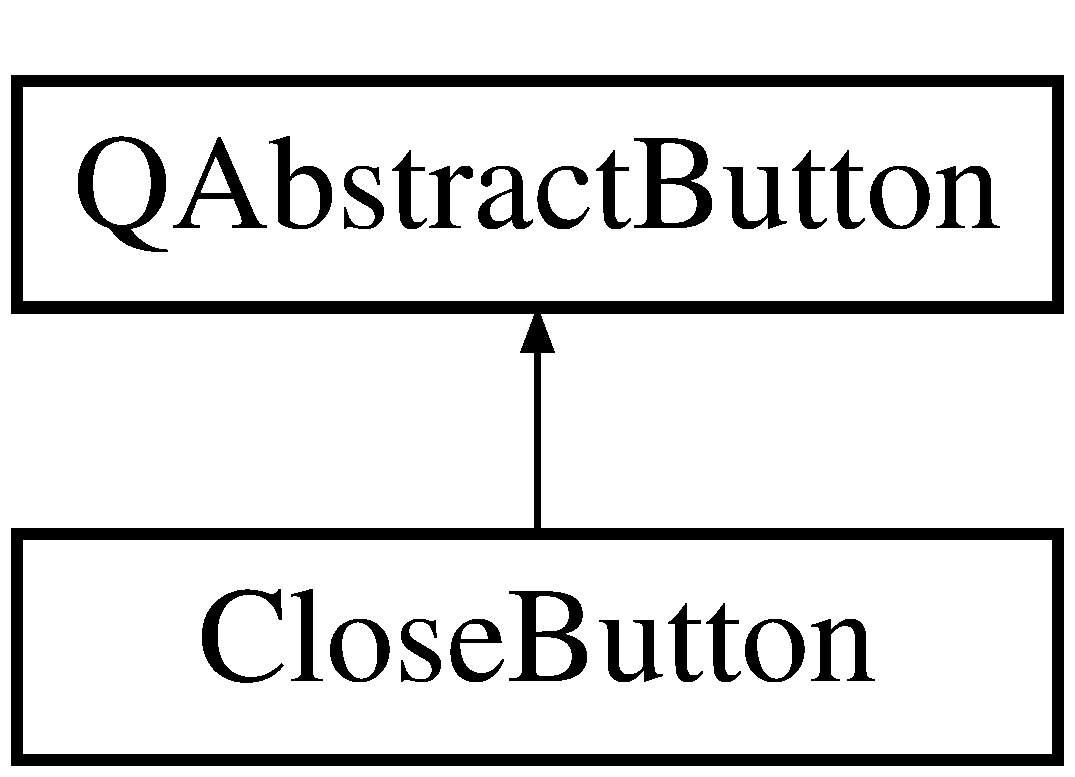
\includegraphics[height=2cm]{class_close_button}
\end{center}
\end{figure}
\subsection*{Public Member Functions}
\begin{DoxyCompactItemize}
\item 
\hypertarget{class_close_button_a51839d4283758bd7221bafe64d08073b}{
{\bfseries CloseButton} (\hyperlink{class_q_widget}{QWidget} $\ast$parent=0)}
\label{class_close_button_a51839d4283758bd7221bafe64d08073b}

\item 
\hypertarget{class_close_button_a468e5cea5ea5f11477651a3c66f38f67}{
QSize {\bfseries sizeHint} () const }
\label{class_close_button_a468e5cea5ea5f11477651a3c66f38f67}

\item 
\hypertarget{class_close_button_a481ecf1d325b880fbedd34c02d2ad566}{
QSize {\bfseries minimumSizeHint} () const }
\label{class_close_button_a481ecf1d325b880fbedd34c02d2ad566}

\item 
\hypertarget{class_close_button_acf50f097face931a52329e1e5e8aeddd}{
void {\bfseries enterEvent} (QEvent $\ast$event)}
\label{class_close_button_acf50f097face931a52329e1e5e8aeddd}

\item 
\hypertarget{class_close_button_abdbde1a235729d0f245ede0d8056c809}{
void {\bfseries leaveEvent} (QEvent $\ast$event)}
\label{class_close_button_abdbde1a235729d0f245ede0d8056c809}

\item 
\hypertarget{class_close_button_ae0531ab78ea9542c1a261ab4d0d8125b}{
void {\bfseries paintEvent} (QPaintEvent $\ast$event)}
\label{class_close_button_ae0531ab78ea9542c1a261ab4d0d8125b}

\end{DoxyCompactItemize}


\subsection{Detailed Description}
Class for close button on tabs $\ast$ taken from qtabbar.cpp. 

The documentation for this class was generated from the following file:\begin{DoxyCompactItemize}
\item 
E:/Programming/QupZilla-\/Project/qupzilla/src/lib/tabwidget/combotabbar.h\end{DoxyCompactItemize}

\hypertarget{class_combo_tab_bar}{
\section{ComboTabBar Class Reference}
\label{class_combo_tab_bar}\index{ComboTabBar@{ComboTabBar}}
}


The \hyperlink{class_combo_tab_bar}{ComboTabBar} class is mixed of a pinned tabbar and a normal scrollable tabbar.  




{\ttfamily \#include $<$combotabbar.h$>$}

Inheritance diagram for ComboTabBar:\begin{figure}[H]
\begin{center}
\leavevmode
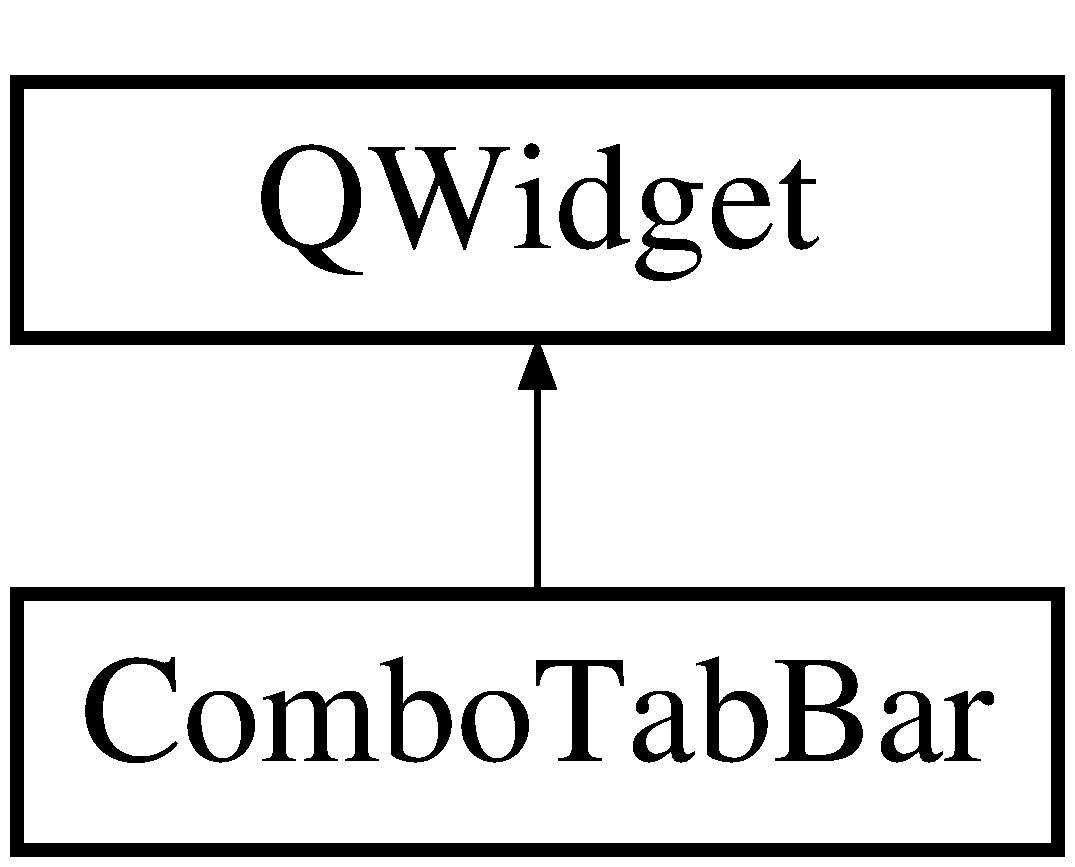
\includegraphics[height=2cm]{class_combo_tab_bar}
\end{center}
\end{figure}
\subsection*{Public Types}
\begin{DoxyCompactItemize}
\item 
enum \hyperlink{class_combo_tab_bar_a1b4d1e5b7dbc95dcf040b481e00760bc}{SizeType} \{ \par
{\bfseries PinnedTabWidth}, 
{\bfseries ActiveTabMinimumWidth}, 
{\bfseries NormalTabMinimumWidth}, 
{\bfseries NormalTabMaximumWidth}, 
\par
{\bfseries OverflowedTabWidth}, 
\hyperlink{class_combo_tab_bar_a1b4d1e5b7dbc95dcf040b481e00760bcaad4e405225830026a514d146b600b955}{ExtraReservedWidth}
 \}
\end{DoxyCompactItemize}
\subsection*{Public Slots}
\begin{DoxyCompactItemize}
\item 
\hypertarget{class_combo_tab_bar_a9cacd6e9340dfff7f356ad28b9e71030}{
void {\bfseries setUpLayout} ()}
\label{class_combo_tab_bar_a9cacd6e9340dfff7f356ad28b9e71030}

\item 
void \hyperlink{class_combo_tab_bar_a67abbf211f68ffe53c10654311a95621}{ensureVisible} (int index=-\/1, int xmargin=-\/1)
\item 
\hypertarget{class_combo_tab_bar_af87d91e7b17e8d5f192f7f0b89c26047}{
void {\bfseries setCurrentIndex} (int index)}
\label{class_combo_tab_bar_af87d91e7b17e8d5f192f7f0b89c26047}

\end{DoxyCompactItemize}
\subsection*{Signals}
\begin{DoxyCompactItemize}
\item 
\hypertarget{class_combo_tab_bar_a94f5ffd04222be4711aa86c43dd8c2c8}{
void {\bfseries overFlowChanged} (bool overFlow)}
\label{class_combo_tab_bar_a94f5ffd04222be4711aa86c43dd8c2c8}

\item 
\hypertarget{class_combo_tab_bar_a809f0e76133375268a91fab6764f8974}{
void {\bfseries currentChanged} (int index)}
\label{class_combo_tab_bar_a809f0e76133375268a91fab6764f8974}

\item 
\hypertarget{class_combo_tab_bar_a109612f4651a809579d58e214693ec4b}{
void {\bfseries tabCloseRequested} (int index)}
\label{class_combo_tab_bar_a109612f4651a809579d58e214693ec4b}

\item 
\hypertarget{class_combo_tab_bar_a996feb2cdfac31b11b4862a889ca1578}{
void {\bfseries tabMoved} (int from, int to)}
\label{class_combo_tab_bar_a996feb2cdfac31b11b4862a889ca1578}

\item 
\hypertarget{class_combo_tab_bar_a4f8d44211878ebcbaa83c6f410a6d6c3}{
void {\bfseries scrollBarValueChanged} (int value)}
\label{class_combo_tab_bar_a4f8d44211878ebcbaa83c6f410a6d6c3}

\end{DoxyCompactItemize}
\subsection*{Public Member Functions}
\begin{DoxyCompactItemize}
\item 
\hypertarget{class_combo_tab_bar_ad215b46a7b36de7254e84a5faeda3271}{
{\bfseries ComboTabBar} (\hyperlink{class_q_widget}{QWidget} $\ast$parent=0)}
\label{class_combo_tab_bar_ad215b46a7b36de7254e84a5faeda3271}

\item 
\hypertarget{class_combo_tab_bar_a0778ead49aac16e76a52e064d4456e38}{
int {\bfseries addTab} (const QString \&text)}
\label{class_combo_tab_bar_a0778ead49aac16e76a52e064d4456e38}

\item 
\hypertarget{class_combo_tab_bar_aa9d7ea42b1140110816427d054573c22}{
int {\bfseries addTab} (const QIcon \&icon, const QString \&text)}
\label{class_combo_tab_bar_aa9d7ea42b1140110816427d054573c22}

\item 
\hypertarget{class_combo_tab_bar_a217ce12ede48579d0093224c056bc22b}{
int {\bfseries insertTab} (int index, const QString \&text)}
\label{class_combo_tab_bar_a217ce12ede48579d0093224c056bc22b}

\item 
\hypertarget{class_combo_tab_bar_aadb37fbf2993cb630e38f1e5e8babb9f}{
int {\bfseries insertTab} (int index, const QIcon \&icon, const QString \&text, bool pinned=false)}
\label{class_combo_tab_bar_aadb37fbf2993cb630e38f1e5e8babb9f}

\item 
\hypertarget{class_combo_tab_bar_a4ea37ffc1a20344bb381ebe476290c73}{
void {\bfseries removeTab} (int index)}
\label{class_combo_tab_bar_a4ea37ffc1a20344bb381ebe476290c73}

\item 
\hypertarget{class_combo_tab_bar_a3461f38651ae174bd65fe74c2afb74a1}{
void {\bfseries moveTab} (int from, int to)}
\label{class_combo_tab_bar_a3461f38651ae174bd65fe74c2afb74a1}

\item 
\hypertarget{class_combo_tab_bar_aa0a9af0b7c063804dd7e7c5a2f410e6a}{
bool {\bfseries isTabEnabled} (int index) const }
\label{class_combo_tab_bar_aa0a9af0b7c063804dd7e7c5a2f410e6a}

\item 
\hypertarget{class_combo_tab_bar_adec9ff85e73e28ca1446a5ed906a9465}{
void {\bfseries setTabEnabled} (int index, bool enabled)}
\label{class_combo_tab_bar_adec9ff85e73e28ca1446a5ed906a9465}

\item 
\hypertarget{class_combo_tab_bar_afc67238651ecdce59e33503618580137}{
QColor {\bfseries tabTextColor} (int index) const }
\label{class_combo_tab_bar_afc67238651ecdce59e33503618580137}

\item 
\hypertarget{class_combo_tab_bar_a6634e7fb2e38f48daa439a89db5c24af}{
void {\bfseries setTabTextColor} (int index, const QColor \&color)}
\label{class_combo_tab_bar_a6634e7fb2e38f48daa439a89db5c24af}

\item 
\hypertarget{class_combo_tab_bar_a2301662a027572fb685937a717a05f7b}{
QRect {\bfseries tabRect} (int index) const }
\label{class_combo_tab_bar_a2301662a027572fb685937a717a05f7b}

\item 
int \hyperlink{class_combo_tab_bar_a2ba10737ac0dd8848f97434a9c5814f3}{tabAt} (const QPoint \&pos) const 
\item 
bool \hyperlink{class_combo_tab_bar_a737d267e4cd82efad188b2d5ce601810}{emptyArea} (const QPoint \&pos) const 
\item 
\hypertarget{class_combo_tab_bar_aa768d3a41df71b0d3179f529ff1b0a2f}{
int {\bfseries mainTabBarCurrentIndex} () const }
\label{class_combo_tab_bar_aa768d3a41df71b0d3179f529ff1b0a2f}

\item 
\hypertarget{class_combo_tab_bar_a71a77325f22110bf223f2f9e0faf52bd}{
int {\bfseries currentIndex} () const }
\label{class_combo_tab_bar_a71a77325f22110bf223f2f9e0faf52bd}

\item 
\hypertarget{class_combo_tab_bar_ad30535b80bc7a75ea26106218b8f9110}{
int {\bfseries count} () const }
\label{class_combo_tab_bar_ad30535b80bc7a75ea26106218b8f9110}

\item 
\hypertarget{class_combo_tab_bar_a84a0e639e0c7fda3e7d7b8b37aa4c4b0}{
void {\bfseries setDrawBase} (bool drawTheBase)}
\label{class_combo_tab_bar_a84a0e639e0c7fda3e7d7b8b37aa4c4b0}

\item 
\hypertarget{class_combo_tab_bar_a6586b51cbab448ae0b36ed01d9103845}{
bool {\bfseries drawBase} () const }
\label{class_combo_tab_bar_a6586b51cbab448ae0b36ed01d9103845}

\item 
\hypertarget{class_combo_tab_bar_a3522f6e767f5d4d55de994efdcceb352}{
Qt::TextElideMode {\bfseries elideMode} () const }
\label{class_combo_tab_bar_a3522f6e767f5d4d55de994efdcceb352}

\item 
\hypertarget{class_combo_tab_bar_a5756d7f84f613b550078861753512ee5}{
void {\bfseries setElideMode} (Qt::TextElideMode elide)}
\label{class_combo_tab_bar_a5756d7f84f613b550078861753512ee5}

\item 
\hypertarget{class_combo_tab_bar_a1f8455c764f3547adf12e8c5106527dd}{
QString {\bfseries tabText} (int index) const }
\label{class_combo_tab_bar_a1f8455c764f3547adf12e8c5106527dd}

\item 
\hypertarget{class_combo_tab_bar_ab23be3e427bcecdd42cb2a3d3cd892bd}{
void {\bfseries setTabText} (int index, const QString \&text)}
\label{class_combo_tab_bar_ab23be3e427bcecdd42cb2a3d3cd892bd}

\item 
\hypertarget{class_combo_tab_bar_a99b60793e4feb4358c7993dddd07333f}{
void {\bfseries setTabToolTip} (int index, const QString \&tip)}
\label{class_combo_tab_bar_a99b60793e4feb4358c7993dddd07333f}

\item 
\hypertarget{class_combo_tab_bar_a1070e2666aa5bed589ef3640ae7a2b78}{
QString {\bfseries tabToolTip} (int index) const }
\label{class_combo_tab_bar_a1070e2666aa5bed589ef3640ae7a2b78}

\item 
\hypertarget{class_combo_tab_bar_aab097d0b41ae4915544eaead6e3d87fc}{
bool {\bfseries tabsClosable} () const }
\label{class_combo_tab_bar_aab097d0b41ae4915544eaead6e3d87fc}

\item 
\hypertarget{class_combo_tab_bar_ac4178c65419140ea5cef414d86167157}{
void {\bfseries setTabsClosable} (bool closable)}
\label{class_combo_tab_bar_ac4178c65419140ea5cef414d86167157}

\item 
\hypertarget{class_combo_tab_bar_a7859982ef655a22efb3d694437d20cd3}{
void {\bfseries setTabButton} (int index, QTabBar::ButtonPosition position, \hyperlink{class_q_widget}{QWidget} $\ast$widget)}
\label{class_combo_tab_bar_a7859982ef655a22efb3d694437d20cd3}

\item 
\hypertarget{class_combo_tab_bar_ad5f5c72528c099547dcd4d76883cac34}{
\hyperlink{class_q_widget}{QWidget} $\ast$ {\bfseries tabButton} (int index, QTabBar::ButtonPosition position) const }
\label{class_combo_tab_bar_ad5f5c72528c099547dcd4d76883cac34}

\item 
\hypertarget{class_combo_tab_bar_a12be78eb2cccb159886662948729f40b}{
QTabBar::SelectionBehavior {\bfseries selectionBehaviorOnRemove} () const }
\label{class_combo_tab_bar_a12be78eb2cccb159886662948729f40b}

\item 
\hypertarget{class_combo_tab_bar_a82daa9a45f727324ab5116288f19e33b}{
void {\bfseries setSelectionBehaviorOnRemove} (QTabBar::SelectionBehavior behavior)}
\label{class_combo_tab_bar_a82daa9a45f727324ab5116288f19e33b}

\item 
\hypertarget{class_combo_tab_bar_a71f4f34d1dc4701d3e6ca51c1c460479}{
bool {\bfseries expanding} () const }
\label{class_combo_tab_bar_a71f4f34d1dc4701d3e6ca51c1c460479}

\item 
\hypertarget{class_combo_tab_bar_a565062955f4c49d62498a7f542a7cdd3}{
void {\bfseries setExpanding} (bool enabled)}
\label{class_combo_tab_bar_a565062955f4c49d62498a7f542a7cdd3}

\item 
\hypertarget{class_combo_tab_bar_ac1892c7f5c092995acd1f2efb8911a66}{
bool {\bfseries isMovable} () const }
\label{class_combo_tab_bar_ac1892c7f5c092995acd1f2efb8911a66}

\item 
\hypertarget{class_combo_tab_bar_a0e551055d8ac21acb511fbc54b9218a8}{
void {\bfseries setMovable} (bool movable)}
\label{class_combo_tab_bar_a0e551055d8ac21acb511fbc54b9218a8}

\item 
\hypertarget{class_combo_tab_bar_a72020d7411a8fed3927e4bef752cccf7}{
bool {\bfseries documentMode} () const }
\label{class_combo_tab_bar_a72020d7411a8fed3927e4bef752cccf7}

\item 
\hypertarget{class_combo_tab_bar_ae63a0415722d0a9e7cb078f67fb5ce8e}{
void {\bfseries setDocumentMode} (bool set)}
\label{class_combo_tab_bar_ae63a0415722d0a9e7cb078f67fb5ce8e}

\item 
\hypertarget{class_combo_tab_bar_ad14aa7e400982a67345b64abb1e9b82d}{
int {\bfseries pinnedTabsCount} () const }
\label{class_combo_tab_bar_ad14aa7e400982a67345b64abb1e9b82d}

\item 
\hypertarget{class_combo_tab_bar_a190dfb072e02cd1064952881dc582ae3}{
int {\bfseries normalTabsCount} () const }
\label{class_combo_tab_bar_a190dfb072e02cd1064952881dc582ae3}

\item 
\hypertarget{class_combo_tab_bar_a9c4413dce9ceba2b42f4cb9fe2eb6c03}{
bool {\bfseries isPinned} (int index) const }
\label{class_combo_tab_bar_a9c4413dce9ceba2b42f4cb9fe2eb6c03}

\item 
\hypertarget{class_combo_tab_bar_ac6f8d027c5eb9eb4976b7f26460749b2}{
void {\bfseries setObjectName} (const QString \&name)}
\label{class_combo_tab_bar_ac6f8d027c5eb9eb4976b7f26460749b2}

\item 
\hypertarget{class_combo_tab_bar_a239981b4576b3bf469e88c950cdf9379}{
void {\bfseries setMouseTracking} (bool enable)}
\label{class_combo_tab_bar_a239981b4576b3bf469e88c950cdf9379}

\item 
\hypertarget{class_combo_tab_bar_ae7a4dde371b625f854275f230520609b}{
void {\bfseries insertCloseButton} (int index)}
\label{class_combo_tab_bar_ae7a4dde371b625f854275f230520609b}

\item 
\hypertarget{class_combo_tab_bar_aad29454b7b4152316af1bceec0ea65d1}{
void {\bfseries setCloseButtonsToolTip} (const QString \&tip)}
\label{class_combo_tab_bar_aad29454b7b4152316af1bceec0ea65d1}

\item 
\hypertarget{class_combo_tab_bar_a6fabbea88ffb64b3c3767f2b40d66174}{
void {\bfseries enableBluredBackground} (bool enable)}
\label{class_combo_tab_bar_a6fabbea88ffb64b3c3767f2b40d66174}

\item 
\hypertarget{class_combo_tab_bar_a75522212d8babac303f31b5aca1f855f}{
QTabBar::ButtonPosition {\bfseries iconButtonPosition} ()}
\label{class_combo_tab_bar_a75522212d8babac303f31b5aca1f855f}

\item 
\hypertarget{class_combo_tab_bar_a1c8c4005030156e07db4b49ab5324714}{
QTabBar::ButtonPosition {\bfseries closeButtonPosition} ()}
\label{class_combo_tab_bar_a1c8c4005030156e07db4b49ab5324714}

\item 
\hypertarget{class_combo_tab_bar_ac3ba8a576a1bde1b246701f4c1708232}{
bool {\bfseries validIndex} (int index) const }
\label{class_combo_tab_bar_ac3ba8a576a1bde1b246701f4c1708232}

\item 
\hypertarget{class_combo_tab_bar_aeef10920a84647ed1b457b8b9cfb19a9}{
void {\bfseries setCurrentNextEnabledIndex} (int offset)}
\label{class_combo_tab_bar_aeef10920a84647ed1b457b8b9cfb19a9}

\item 
\hypertarget{class_combo_tab_bar_a380190b950a2070287ee79cf8ff3b47d}{
bool {\bfseries usesScrollButtons} () const }
\label{class_combo_tab_bar_a380190b950a2070287ee79cf8ff3b47d}

\item 
\hypertarget{class_combo_tab_bar_ad2fd8ce2abc792dca03735ff81c5d47e}{
void {\bfseries setUsesScrollButtons} (bool useButtons)}
\label{class_combo_tab_bar_ad2fd8ce2abc792dca03735ff81c5d47e}

\item 
\hypertarget{class_combo_tab_bar_a033143d446119c9145bb4ee04599c057}{
bool {\bfseries isDragInProgress} () const }
\label{class_combo_tab_bar_a033143d446119c9145bb4ee04599c057}

\item 
\hypertarget{class_combo_tab_bar_a3fdc1a1707a2e2b6c46340884fad4065}{
bool {\bfseries isMainBarOverflowed} () const }
\label{class_combo_tab_bar_a3fdc1a1707a2e2b6c46340884fad4065}

\item 
int \hyperlink{class_combo_tab_bar_add04fdbda2e634592d3ba6c0a3083e46}{cornerWidth} (Qt::Corner corner) const 
\item 
void \hyperlink{class_combo_tab_bar_a3371dbfa9365711b28f7440dbd4d36e6}{addCornerWidget} (\hyperlink{class_q_widget}{QWidget} $\ast$widget, Qt::Corner corner)
\end{DoxyCompactItemize}
\subsection*{Protected Member Functions}
\begin{DoxyCompactItemize}
\item 
\hypertarget{class_combo_tab_bar_abe7ceb107e863285c858cb24bc895844}{
int {\bfseries mainTabBarWidth} () const }
\label{class_combo_tab_bar_abe7ceb107e863285c858cb24bc895844}

\item 
\hypertarget{class_combo_tab_bar_a3509e98c3e69c1f708b342d39aef3e7e}{
int {\bfseries pinTabBarWidth} () const }
\label{class_combo_tab_bar_a3509e98c3e69c1f708b342d39aef3e7e}

\item 
\hypertarget{class_combo_tab_bar_a3d365b44cdd5420ef9237cf483b3aab4}{
void {\bfseries wheelEvent} (QWheelEvent $\ast$event)}
\label{class_combo_tab_bar_a3d365b44cdd5420ef9237cf483b3aab4}

\item 
\hypertarget{class_combo_tab_bar_a5b078b04fc16e00b91fbea9b3c062113}{
void {\bfseries showEvent} (QShowEvent $\ast$event)}
\label{class_combo_tab_bar_a5b078b04fc16e00b91fbea9b3c062113}

\item 
\hypertarget{class_combo_tab_bar_a544941e84284cad88c47eb3d992a0899}{
void {\bfseries enterEvent} (QEvent $\ast$event)}
\label{class_combo_tab_bar_a544941e84284cad88c47eb3d992a0899}

\item 
\hypertarget{class_combo_tab_bar_a6e1abbacc023355aa7db27f1499ef7f3}{
void {\bfseries leaveEvent} (QEvent $\ast$event)}
\label{class_combo_tab_bar_a6e1abbacc023355aa7db27f1499ef7f3}

\item 
\hypertarget{class_combo_tab_bar_a2a1b7d5605c97f99238d2bcbb8ab9c41}{
bool {\bfseries eventFilter} (QObject $\ast$obj, QEvent $\ast$ev)}
\label{class_combo_tab_bar_a2a1b7d5605c97f99238d2bcbb8ab9c41}

\item 
\hypertarget{class_combo_tab_bar_a591bd7d1efe029de98eb6e140286a58d}{
void {\bfseries paintEvent} (QPaintEvent $\ast$ev)}
\label{class_combo_tab_bar_a591bd7d1efe029de98eb6e140286a58d}

\item 
virtual int \hyperlink{class_combo_tab_bar_abfe5f8784d0433283bca4c087f0d2b42}{comboTabBarPixelMetric} (\hyperlink{class_combo_tab_bar_a1b4d1e5b7dbc95dcf040b481e00760bc}{SizeType} sizeType) const 
\item 
virtual QSize \hyperlink{class_combo_tab_bar_aedd5c86124231d4d5df2bbc297edf046}{tabSizeHint} (int index, bool fast=false) const 
\item 
\hypertarget{class_combo_tab_bar_a9d85cfc014fde05f25de00854f3c2fb3}{
virtual void {\bfseries tabInserted} (int index)}
\label{class_combo_tab_bar_a9d85cfc014fde05f25de00854f3c2fb3}

\item 
\hypertarget{class_combo_tab_bar_a81e98edcbd2467a08cf70e8af942a9c7}{
virtual void {\bfseries tabRemoved} (int index)}
\label{class_combo_tab_bar_a81e98edcbd2467a08cf70e8af942a9c7}

\end{DoxyCompactItemize}
\subsection*{Properties}
\begin{DoxyCompactItemize}
\item 
\hypertarget{class_combo_tab_bar_a6c31d71f78a5bec1c76dfb4d266464e3}{
int {\bfseries currentIndex}}
\label{class_combo_tab_bar_a6c31d71f78a5bec1c76dfb4d266464e3}

\item 
\hypertarget{class_combo_tab_bar_afa1a0d26530e0d4d21dee3273abcd831}{
int {\bfseries count}}
\label{class_combo_tab_bar_afa1a0d26530e0d4d21dee3273abcd831}

\end{DoxyCompactItemize}
\subsection*{Private Slots}
\begin{DoxyCompactItemize}
\item 
\hypertarget{class_combo_tab_bar_afe1a53dbe57271afbb725b609d74623a}{
void {\bfseries setMinimumWidths} ()}
\label{class_combo_tab_bar_afe1a53dbe57271afbb725b609d74623a}

\item 
\hypertarget{class_combo_tab_bar_ae8020108ae4d79d1f9337344d4764600}{
void {\bfseries slotCurrentChanged} (int index)}
\label{class_combo_tab_bar_ae8020108ae4d79d1f9337344d4764600}

\item 
\hypertarget{class_combo_tab_bar_afa7c13566d5e9f261b37a37a217a3086}{
void {\bfseries slotTabCloseRequested} (int index)}
\label{class_combo_tab_bar_afa7c13566d5e9f261b37a37a217a3086}

\item 
\hypertarget{class_combo_tab_bar_a29d5becee02b839d98287edd0499ab10}{
void {\bfseries slotTabMoved} (int from, int to)}
\label{class_combo_tab_bar_a29d5becee02b839d98287edd0499ab10}

\item 
\hypertarget{class_combo_tab_bar_ab4a00eed0da98fac7cc68deab83b93b5}{
void {\bfseries closeTabFromButton} ()}
\label{class_combo_tab_bar_ab4a00eed0da98fac7cc68deab83b93b5}

\item 
\hypertarget{class_combo_tab_bar_a0735e73e3f67b34a39237ebb6b6d3040}{
void {\bfseries updateTabBars} ()}
\label{class_combo_tab_bar_a0735e73e3f67b34a39237ebb6b6d3040}

\item 
\hypertarget{class_combo_tab_bar_afca20d3ddbd5220cd1c5abb347d68693}{
void {\bfseries emitOverFlowChanged} ()}
\label{class_combo_tab_bar_afca20d3ddbd5220cd1c5abb347d68693}

\end{DoxyCompactItemize}
\subsection*{Private Member Functions}
\begin{DoxyCompactItemize}
\item 
\hypertarget{class_combo_tab_bar_a3aa53aae4c3040bb27ac6065267b4db1}{
\hyperlink{class_tab_bar_helper}{TabBarHelper} $\ast$ {\bfseries mainTabBar} () const }
\label{class_combo_tab_bar_a3aa53aae4c3040bb27ac6065267b4db1}

\item 
\hyperlink{class_tab_bar_helper}{TabBarHelper} $\ast$ \hyperlink{class_combo_tab_bar_a262d76912a414546f74bb804de6abe9c}{localTabBar} (int index=-\/1) const 
\item 
int \hyperlink{class_combo_tab_bar_ac37381dc0f5d788b9d21508fecec6013}{toLocalIndex} (int globalIndex) const 
\item 
\hypertarget{class_combo_tab_bar_a146ca78e63ab40b476685be5d87166f1}{
void {\bfseries updatePinnedTabBarVisibility} ()}
\label{class_combo_tab_bar_a146ca78e63ab40b476685be5d87166f1}

\end{DoxyCompactItemize}
\subsection*{Private Attributes}
\begin{DoxyCompactItemize}
\item 
\hypertarget{class_combo_tab_bar_acaa83471248b7e20390a8d0e8b9dc27e}{
QHBoxLayout $\ast$ {\bfseries m\_\-mainLayout}}
\label{class_combo_tab_bar_acaa83471248b7e20390a8d0e8b9dc27e}

\item 
\hypertarget{class_combo_tab_bar_afdcf007a49d034baffb3a5794a236381}{
QHBoxLayout $\ast$ {\bfseries m\_\-leftLayout}}
\label{class_combo_tab_bar_afdcf007a49d034baffb3a5794a236381}

\item 
\hypertarget{class_combo_tab_bar_a558bc651311777d9a3ad392b5ddbaa94}{
QHBoxLayout $\ast$ {\bfseries m\_\-rightLayout}}
\label{class_combo_tab_bar_a558bc651311777d9a3ad392b5ddbaa94}

\item 
\hypertarget{class_combo_tab_bar_a6cc9c2a3a16201cd0984f5bd41258042}{
\hyperlink{class_q_widget}{QWidget} $\ast$ {\bfseries m\_\-leftContainer}}
\label{class_combo_tab_bar_a6cc9c2a3a16201cd0984f5bd41258042}

\item 
\hypertarget{class_combo_tab_bar_a66a2efc3eed4095e7f9862656de1a332}{
\hyperlink{class_q_widget}{QWidget} $\ast$ {\bfseries m\_\-rightContainer}}
\label{class_combo_tab_bar_a66a2efc3eed4095e7f9862656de1a332}

\item 
\hypertarget{class_combo_tab_bar_a9dbfacde3077b92ba3044623463b9257}{
\hyperlink{class_tab_bar_helper}{TabBarHelper} $\ast$ {\bfseries m\_\-mainTabBar}}
\label{class_combo_tab_bar_a9dbfacde3077b92ba3044623463b9257}

\item 
\hypertarget{class_combo_tab_bar_a76d46b2305c97bbe34108f12b7a29643}{
\hyperlink{class_tab_bar_helper}{TabBarHelper} $\ast$ {\bfseries m\_\-pinnedTabBar}}
\label{class_combo_tab_bar_a76d46b2305c97bbe34108f12b7a29643}

\item 
\hypertarget{class_combo_tab_bar_a13160404b902adde21884aa1a09c2302}{
\hyperlink{class_tab_bar_scroll_widget}{TabBarScrollWidget} $\ast$ {\bfseries m\_\-mainTabBarWidget}}
\label{class_combo_tab_bar_a13160404b902adde21884aa1a09c2302}

\item 
\hypertarget{class_combo_tab_bar_a6d60e544d64cb0c4610983a3008b6e3a}{
\hyperlink{class_tab_bar_scroll_widget}{TabBarScrollWidget} $\ast$ {\bfseries m\_\-pinnedTabBarWidget}}
\label{class_combo_tab_bar_a6d60e544d64cb0c4610983a3008b6e3a}

\item 
\hypertarget{class_combo_tab_bar_aaa6fd8c84151411f93cbc1909a77410c}{
QString {\bfseries m\_\-closeButtonsToolTip}}
\label{class_combo_tab_bar_aaa6fd8c84151411f93cbc1909a77410c}

\item 
\hypertarget{class_combo_tab_bar_a51e2466e5de0923218a679b0299ea7ec}{
bool {\bfseries m\_\-mainBarOverFlowed}}
\label{class_combo_tab_bar_a51e2466e5de0923218a679b0299ea7ec}

\item 
\hypertarget{class_combo_tab_bar_acf0bfd89fb53d67b4aa02d4a992bae25}{
bool {\bfseries m\_\-lastAppliedOverflow}}
\label{class_combo_tab_bar_acf0bfd89fb53d67b4aa02d4a992bae25}

\item 
\hypertarget{class_combo_tab_bar_ab5f03aa77a741a36934334176badccaf}{
bool {\bfseries m\_\-usesScrollButtons}}
\label{class_combo_tab_bar_ab5f03aa77a741a36934334176badccaf}

\item 
\hypertarget{class_combo_tab_bar_a994055730c9a831aab48cee1ec91d74f}{
bool {\bfseries m\_\-bluredBackground}}
\label{class_combo_tab_bar_a994055730c9a831aab48cee1ec91d74f}

\item 
\hypertarget{class_combo_tab_bar_aaa4bb25bb3d32e338697d4c317d6135a}{
bool {\bfseries m\_\-blockCurrentChangedSignal}}
\label{class_combo_tab_bar_aaa4bb25bb3d32e338697d4c317d6135a}

\end{DoxyCompactItemize}
\subsection*{Friends}
\begin{DoxyCompactItemize}
\item 
\hypertarget{class_combo_tab_bar_a2c48367f51e58bbeaea3140bd86b5326}{
class \hyperlink{class_combo_tab_bar_a2c48367f51e58bbeaea3140bd86b5326}{TabBarHelper}}
\label{class_combo_tab_bar_a2c48367f51e58bbeaea3140bd86b5326}

\item 
\hypertarget{class_combo_tab_bar_ab30c27851131b8d8bec48bee17832d43}{
class \hyperlink{class_combo_tab_bar_ab30c27851131b8d8bec48bee17832d43}{TabStackedWidget}}
\label{class_combo_tab_bar_ab30c27851131b8d8bec48bee17832d43}

\end{DoxyCompactItemize}


\subsection{Detailed Description}
The \hyperlink{class_combo_tab_bar}{ComboTabBar} class is mixed of a pinned tabbar and a normal scrollable tabbar. It has a horizontal layout containing: m\_\-leftContainer $|$ m\_\-pinnedTabBarWidget $|$ m\_\-mainTabBarWidget $|$ m\_\-rightContainer


\begin{DoxyItemize}
\item Left/Right Containers: Use \hyperlink{class_combo_tab_bar_a3371dbfa9365711b28f7440dbd4d36e6}{addCornerWidget()} to add widget to m\_\-leftContainer or m\_\-rightContainer
\end{DoxyItemize}


\begin{DoxyItemize}
\item Pinned/Main TabBarWidgets: They are of type \hyperlink{class_tab_bar_scroll_widget}{TabBarScrollWidget}, and they add scrollbar to \hyperlink{class_q_tab_bar}{QTabBar} 
\end{DoxyItemize}

\subsection{Member Enumeration Documentation}
\hypertarget{class_combo_tab_bar_a1b4d1e5b7dbc95dcf040b481e00760bc}{
\index{ComboTabBar@{ComboTabBar}!SizeType@{SizeType}}
\index{SizeType@{SizeType}!ComboTabBar@{ComboTabBar}}
\subsubsection[{SizeType}]{\setlength{\rightskip}{0pt plus 5cm}enum {\bf ComboTabBar::SizeType}}}
\label{class_combo_tab_bar_a1b4d1e5b7dbc95dcf040b481e00760bc}


used by \hyperlink{class_combo_tab_bar_abfe5f8784d0433283bca4c087f0d2b42}{comboTabBarPixelMetric()} 

\begin{Desc}
\item[Enumerator: ]\par
\begin{description}
\index{ExtraReservedWidth@{ExtraReservedWidth}!ComboTabBar@{ComboTabBar}}\index{ComboTabBar@{ComboTabBar}!ExtraReservedWidth@{ExtraReservedWidth}}\item[{\em 
\hypertarget{class_combo_tab_bar_a1b4d1e5b7dbc95dcf040b481e00760bcaad4e405225830026a514d146b600b955}{
ExtraReservedWidth}
\label{class_combo_tab_bar_a1b4d1e5b7dbc95dcf040b481e00760bcaad4e405225830026a514d146b600b955}
}]e.g.: reserved space for \char`\"{}add tab\char`\"{} and \char`\"{}list tab\char`\"{} buttons \end{description}
\end{Desc}



\subsection{Member Function Documentation}
\hypertarget{class_combo_tab_bar_a3371dbfa9365711b28f7440dbd4d36e6}{
\index{ComboTabBar@{ComboTabBar}!addCornerWidget@{addCornerWidget}}
\index{addCornerWidget@{addCornerWidget}!ComboTabBar@{ComboTabBar}}
\subsubsection[{addCornerWidget}]{\setlength{\rightskip}{0pt plus 5cm}void ComboTabBar::addCornerWidget ({\bf QWidget} $\ast$ {\em widget}, \/  Qt::Corner {\em corner})}}
\label{class_combo_tab_bar_a3371dbfa9365711b28f7440dbd4d36e6}


Add widget to the left/right corner. 

\hypertarget{class_combo_tab_bar_abfe5f8784d0433283bca4c087f0d2b42}{
\index{ComboTabBar@{ComboTabBar}!comboTabBarPixelMetric@{comboTabBarPixelMetric}}
\index{comboTabBarPixelMetric@{comboTabBarPixelMetric}!ComboTabBar@{ComboTabBar}}
\subsubsection[{comboTabBarPixelMetric}]{\setlength{\rightskip}{0pt plus 5cm}virtual int ComboTabBar::comboTabBarPixelMetric ({\bf SizeType} {\em sizeType}) const\hspace{0.3cm}{\ttfamily  \mbox{[}protected, virtual\mbox{]}}}}
\label{class_combo_tab_bar_abfe5f8784d0433283bca4c087f0d2b42}


should returns width for each SizeType, if UI is not completely initialized then it have to return -\/1 (at least for PinnedTabWidth) 

\hypertarget{class_combo_tab_bar_add04fdbda2e634592d3ba6c0a3083e46}{
\index{ComboTabBar@{ComboTabBar}!cornerWidth@{cornerWidth}}
\index{cornerWidth@{cornerWidth}!ComboTabBar@{ComboTabBar}}
\subsubsection[{cornerWidth}]{\setlength{\rightskip}{0pt plus 5cm}int ComboTabBar::cornerWidth (Qt::Corner {\em corner}) const}}
\label{class_combo_tab_bar_add04fdbda2e634592d3ba6c0a3083e46}


Width of all widgets in the corner. 

\hypertarget{class_combo_tab_bar_a737d267e4cd82efad188b2d5ce601810}{
\index{ComboTabBar@{ComboTabBar}!emptyArea@{emptyArea}}
\index{emptyArea@{emptyArea}!ComboTabBar@{ComboTabBar}}
\subsubsection[{emptyArea}]{\setlength{\rightskip}{0pt plus 5cm}bool ComboTabBar::emptyArea (const QPoint \& {\em pos}) const}}
\label{class_combo_tab_bar_a737d267e4cd82efad188b2d5ce601810}


Returns true if there is an empty area at pos (returns false if there are buttons or other widgets on the pos). 

\hypertarget{class_combo_tab_bar_a67abbf211f68ffe53c10654311a95621}{
\index{ComboTabBar@{ComboTabBar}!ensureVisible@{ensureVisible}}
\index{ensureVisible@{ensureVisible}!ComboTabBar@{ComboTabBar}}
\subsubsection[{ensureVisible}]{\setlength{\rightskip}{0pt plus 5cm}void ComboTabBar::ensureVisible (int {\em index} = {\ttfamily -\/1}, \/  int {\em xmargin} = {\ttfamily -\/1})\hspace{0.3cm}{\ttfamily  \mbox{[}slot\mbox{]}}}}
\label{class_combo_tab_bar_a67abbf211f68ffe53c10654311a95621}


scrolls to index or currentIndex() if index is -\/1 (default) 

\hypertarget{class_combo_tab_bar_a262d76912a414546f74bb804de6abe9c}{
\index{ComboTabBar@{ComboTabBar}!localTabBar@{localTabBar}}
\index{localTabBar@{localTabBar}!ComboTabBar@{ComboTabBar}}
\subsubsection[{localTabBar}]{\setlength{\rightskip}{0pt plus 5cm}{\bf TabBarHelper}$\ast$ ComboTabBar::localTabBar (int {\em index} = {\ttfamily -\/1}) const\hspace{0.3cm}{\ttfamily  \mbox{[}private\mbox{]}}}}
\label{class_combo_tab_bar_a262d76912a414546f74bb804de6abe9c}


returns internal \hyperlink{class_tab_bar_helper}{TabBarHelper} related to index 

\hypertarget{class_combo_tab_bar_a2ba10737ac0dd8848f97434a9c5814f3}{
\index{ComboTabBar@{ComboTabBar}!tabAt@{tabAt}}
\index{tabAt@{tabAt}!ComboTabBar@{ComboTabBar}}
\subsubsection[{tabAt}]{\setlength{\rightskip}{0pt plus 5cm}int ComboTabBar::tabAt (const QPoint \& {\em pos}) const}}
\label{class_combo_tab_bar_a2ba10737ac0dd8848f97434a9c5814f3}


Returns tab index at pos, or -\/1. 

\hypertarget{class_combo_tab_bar_aedd5c86124231d4d5df2bbc297edf046}{
\index{ComboTabBar@{ComboTabBar}!tabSizeHint@{tabSizeHint}}
\index{tabSizeHint@{tabSizeHint}!ComboTabBar@{ComboTabBar}}
\subsubsection[{tabSizeHint}]{\setlength{\rightskip}{0pt plus 5cm}virtual QSize ComboTabBar::tabSizeHint (int {\em index}, \/  bool {\em fast} = {\ttfamily false}) const\hspace{0.3cm}{\ttfamily  \mbox{[}protected, virtual\mbox{]}}}}
\label{class_combo_tab_bar_aedd5c86124231d4d5df2bbc297edf046}


Notice: Use \char`\"{}fast = true\char`\"{} when all pinned tabs have the same size, and also all normal tabs have the same size. 

\hypertarget{class_combo_tab_bar_ac37381dc0f5d788b9d21508fecec6013}{
\index{ComboTabBar@{ComboTabBar}!toLocalIndex@{toLocalIndex}}
\index{toLocalIndex@{toLocalIndex}!ComboTabBar@{ComboTabBar}}
\subsubsection[{toLocalIndex}]{\setlength{\rightskip}{0pt plus 5cm}int ComboTabBar::toLocalIndex (int {\em globalIndex}) const\hspace{0.3cm}{\ttfamily  \mbox{[}private\mbox{]}}}}
\label{class_combo_tab_bar_ac37381dc0f5d788b9d21508fecec6013}


translate globalIndex(=index related to \hyperlink{class_combo_tab_bar}{ComboTabBar}) to localIndex(=index related to internal \hyperlink{class_tab_bar_helper}{TabBarHelper}) 



The documentation for this class was generated from the following file:\begin{DoxyCompactItemize}
\item 
E:/Programming/QupZilla-\/Project/qupzilla/src/lib/tabwidget/combotabbar.h\end{DoxyCompactItemize}

\hypertarget{class_q_abstract_button}{
\section{QAbstractButton Class Reference}
\label{class_q_abstract_button}\index{QAbstractButton@{QAbstractButton}}
}
Inheritance diagram for QAbstractButton:\begin{figure}[H]
\begin{center}
\leavevmode
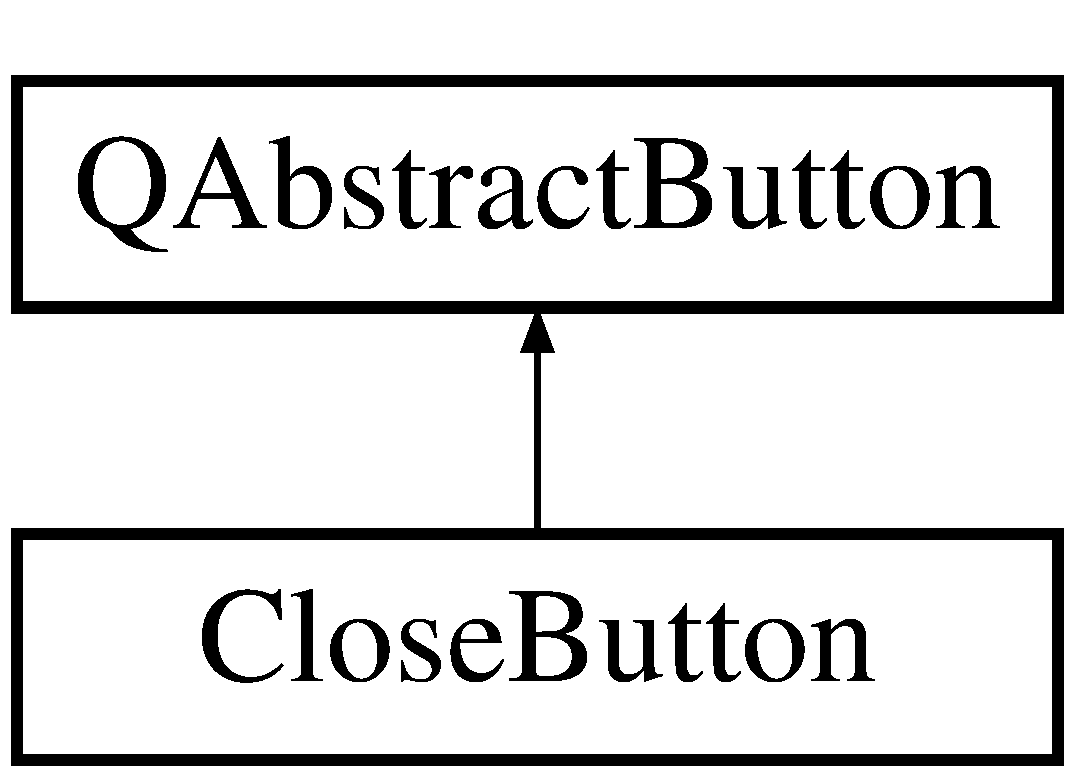
\includegraphics[height=2cm]{class_q_abstract_button}
\end{center}
\end{figure}


The documentation for this class was generated from the following file:\begin{DoxyCompactItemize}
\item 
E:/Programming/QupZilla-\/Project/qupzilla/src/lib/tabwidget/combotabbar.h\end{DoxyCompactItemize}

\hypertarget{class_q_scroll_bar}{
\section{QScrollBar Class Reference}
\label{class_q_scroll_bar}\index{QScrollBar@{QScrollBar}}
}
Inheritance diagram for QScrollBar:\begin{figure}[H]
\begin{center}
\leavevmode
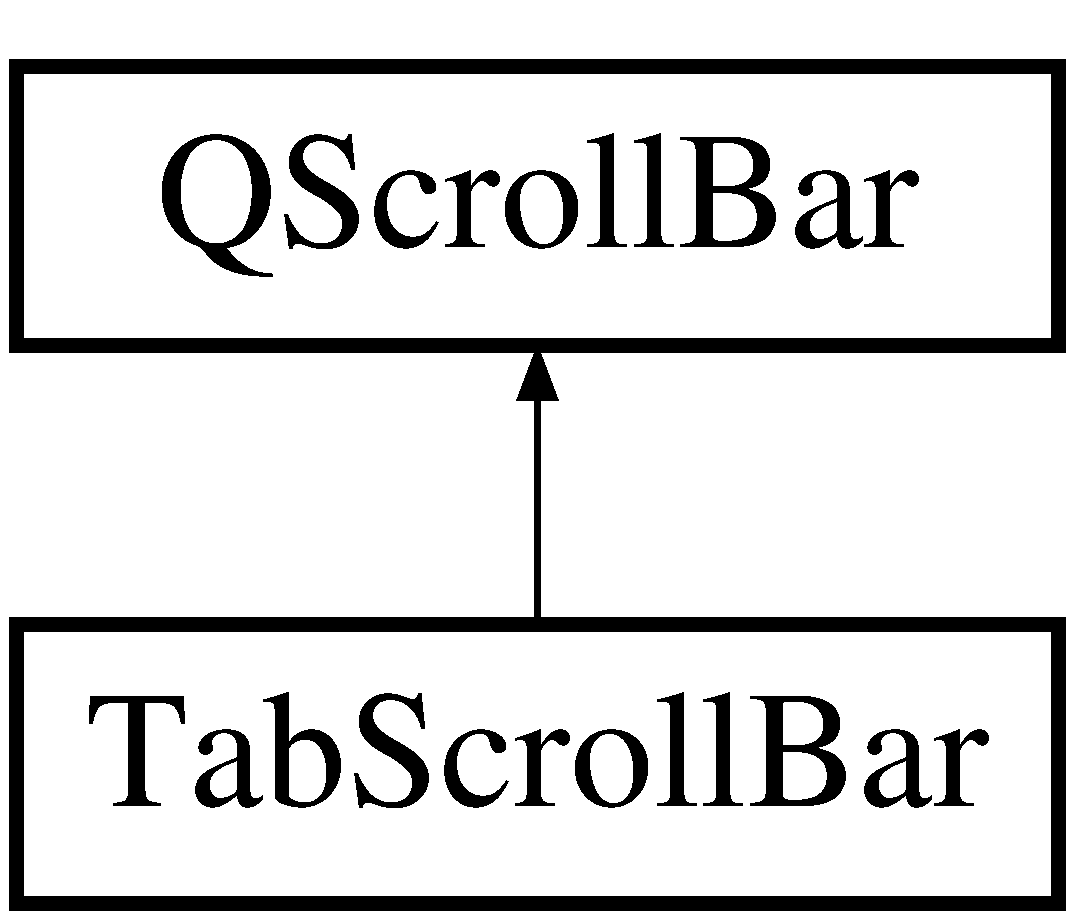
\includegraphics[height=2cm]{class_q_scroll_bar}
\end{center}
\end{figure}


The documentation for this class was generated from the following file:\begin{DoxyCompactItemize}
\item 
E:/Programming/QupZilla-\/Project/qupzilla/src/lib/tabwidget/combotabbar.h\end{DoxyCompactItemize}

\hypertarget{class_q_tab_bar}{
\section{QTabBar Class Reference}
\label{class_q_tab_bar}\index{QTabBar@{QTabBar}}
}
Inheritance diagram for QTabBar:\begin{figure}[H]
\begin{center}
\leavevmode
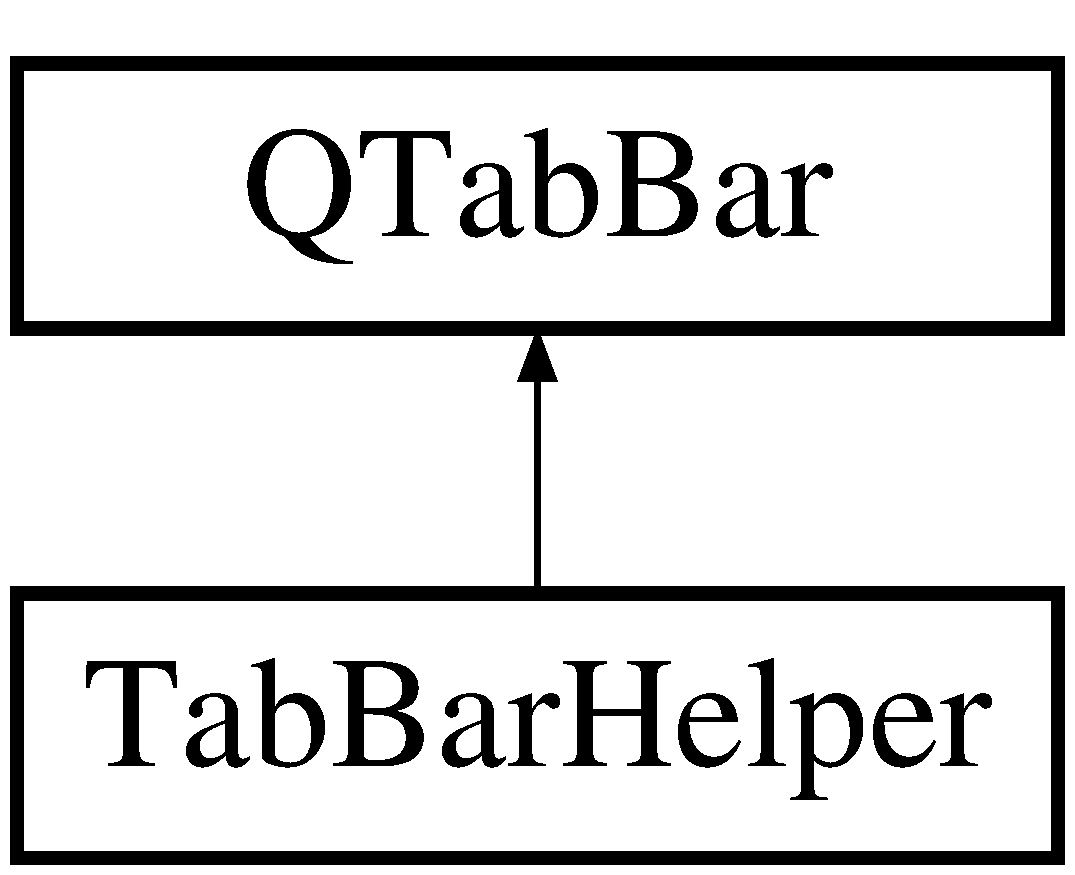
\includegraphics[height=2cm]{class_q_tab_bar}
\end{center}
\end{figure}


The documentation for this class was generated from the following file:\begin{DoxyCompactItemize}
\item 
E:/Programming/QupZilla-\/Project/qupzilla/src/lib/tabwidget/combotabbar.h\end{DoxyCompactItemize}

\hypertarget{class_q_widget}{
\section{QWidget Class Reference}
\label{class_q_widget}\index{QWidget@{QWidget}}
}
Inheritance diagram for QWidget:\begin{figure}[H]
\begin{center}
\leavevmode
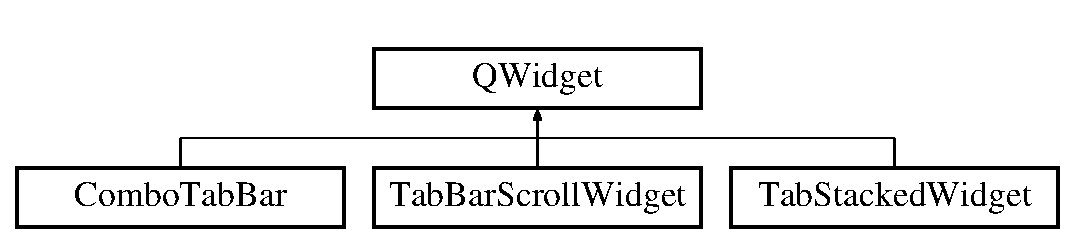
\includegraphics[height=2cm]{class_q_widget}
\end{center}
\end{figure}


The documentation for this class was generated from the following file:\begin{DoxyCompactItemize}
\item 
E:/Programming/QupZilla-\/Project/qupzilla/src/lib/tabwidget/tabstackedwidget.h\end{DoxyCompactItemize}

\hypertarget{class_tab_bar_helper}{
\section{TabBarHelper Class Reference}
\label{class_tab_bar_helper}\index{TabBarHelper@{TabBarHelper}}
}


A subclass of \hyperlink{class_q_tab_bar}{QTabBar} that can be inactivated.  




{\ttfamily \#include $<$combotabbar.h$>$}

Inheritance diagram for TabBarHelper:\begin{figure}[H]
\begin{center}
\leavevmode
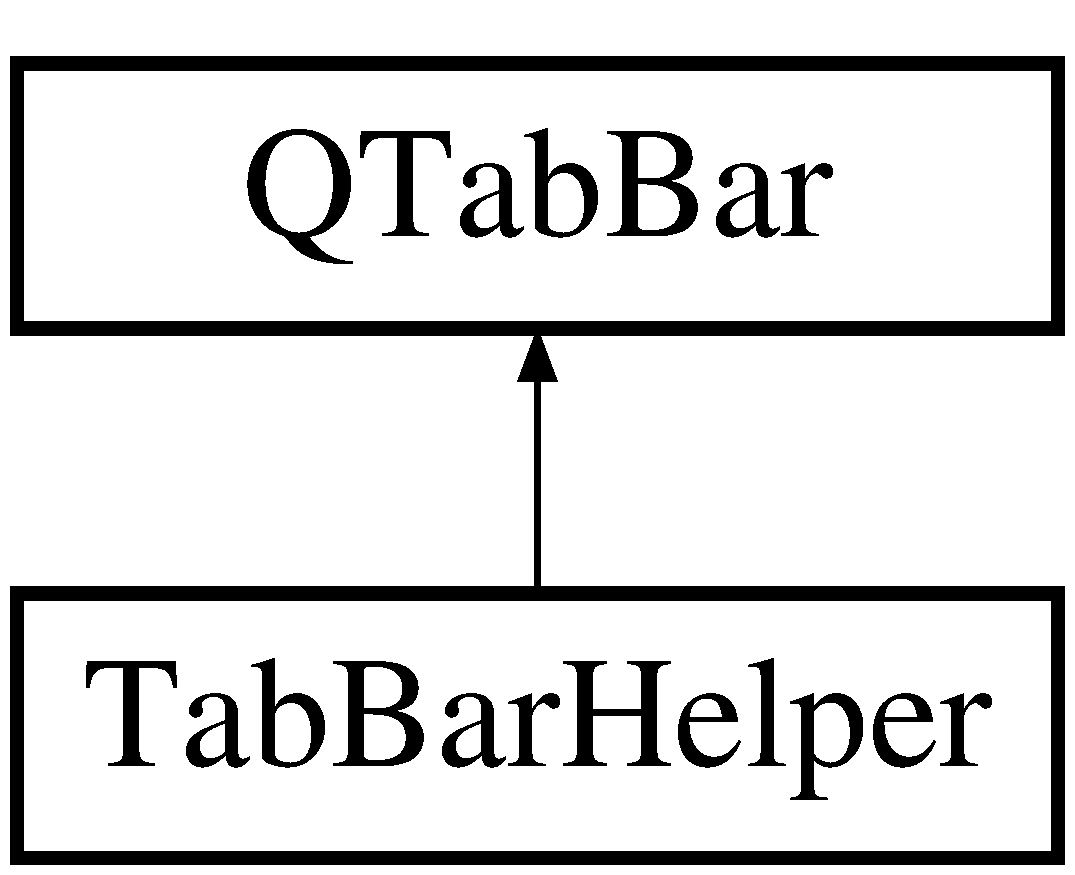
\includegraphics[height=2cm]{class_tab_bar_helper}
\end{center}
\end{figure}
\subsection*{Public Slots}
\begin{DoxyCompactItemize}
\item 
\hypertarget{class_tab_bar_helper_aecf7527d83bce94d0f3b6c985861b003}{
void {\bfseries setCurrentIndex} (int index)}
\label{class_tab_bar_helper_aecf7527d83bce94d0f3b6c985861b003}

\end{DoxyCompactItemize}
\subsection*{Public Member Functions}
\begin{DoxyCompactItemize}
\item 
\hypertarget{class_tab_bar_helper_af9ced889c0be86aefa08d77a70a44bdd}{
{\bfseries TabBarHelper} (bool isPinnedTabBar, \hyperlink{class_combo_tab_bar}{ComboTabBar} $\ast$comboTabBar)}
\label{class_tab_bar_helper_af9ced889c0be86aefa08d77a70a44bdd}

\item 
\hypertarget{class_tab_bar_helper_a28baa6185f46e5db6880ae25a2802307}{
void {\bfseries setTabButton} (int index, QTabBar::ButtonPosition position, \hyperlink{class_q_widget}{QWidget} $\ast$widget)}
\label{class_tab_bar_helper_a28baa6185f46e5db6880ae25a2802307}

\item 
\hypertarget{class_tab_bar_helper_a730752cb66f05baea1796c694051cb0a}{
QSize {\bfseries tabSizeHint} (int index) const }
\label{class_tab_bar_helper_a730752cb66f05baea1796c694051cb0a}

\item 
\hypertarget{class_tab_bar_helper_ac33cf816a8ed021905044dc04d823c4e}{
QSize {\bfseries baseClassTabSizeHint} (int index) const }
\label{class_tab_bar_helper_ac33cf816a8ed021905044dc04d823c4e}

\item 
\hypertarget{class_tab_bar_helper_abcc45aacfb483444d03f1c9bf3b9ea6f}{
bool {\bfseries isActiveTabBar} ()}
\label{class_tab_bar_helper_abcc45aacfb483444d03f1c9bf3b9ea6f}

\item 
\hypertarget{class_tab_bar_helper_aa93e42dcc138bf87905524ec854bfc3b}{
void {\bfseries setActiveTabBar} (bool activate)}
\label{class_tab_bar_helper_aa93e42dcc138bf87905524ec854bfc3b}

\item 
\hypertarget{class_tab_bar_helper_ae3b64c247a7953682dd1fc53b784d5dc}{
void {\bfseries removeTab} (int index)}
\label{class_tab_bar_helper_ae3b64c247a7953682dd1fc53b784d5dc}

\item 
\hypertarget{class_tab_bar_helper_a11e0dba4a8d1547a2b0ed4898a2573ef}{
void {\bfseries setScrollArea} (QScrollArea $\ast$scrollArea)}
\label{class_tab_bar_helper_a11e0dba4a8d1547a2b0ed4898a2573ef}

\item 
\hypertarget{class_tab_bar_helper_a3dd9da07487a7549d69c80380fc83951}{
void {\bfseries useFastTabSizeHint} (bool enabled)}
\label{class_tab_bar_helper_a3dd9da07487a7549d69c80380fc83951}

\item 
\hypertarget{class_tab_bar_helper_a21dac47e89bca9dc01d515763fe9af37}{
bool {\bfseries isDisplayedOnViewPort} (int globalLeft, int globalRight)}
\label{class_tab_bar_helper_a21dac47e89bca9dc01d515763fe9af37}

\item 
\hypertarget{class_tab_bar_helper_ad9fefe50279cc163e20647dd6ef220c6}{
bool {\bfseries isDragInProgress} () const }
\label{class_tab_bar_helper_ad9fefe50279cc163e20647dd6ef220c6}

\item 
\hypertarget{class_tab_bar_helper_ab071cb66c0d3c64e04bb84859bf45bc2}{
void {\bfseries enableBluredBackground} (bool enable)}
\label{class_tab_bar_helper_ab071cb66c0d3c64e04bb84859bf45bc2}

\end{DoxyCompactItemize}
\subsection*{Static Public Member Functions}
\begin{DoxyCompactItemize}
\item 
\hypertarget{class_tab_bar_helper_a83a02154b55440c34316916475c40f6a}{
static void {\bfseries initStyleBaseOption} (QStyleOptionTabBarBaseV2 $\ast$optTabBase, \hyperlink{class_q_tab_bar}{QTabBar} $\ast$tabbar, QSize size)}
\label{class_tab_bar_helper_a83a02154b55440c34316916475c40f6a}

\end{DoxyCompactItemize}
\subsection*{Private Slots}
\begin{DoxyCompactItemize}
\item 
\hypertarget{class_tab_bar_helper_a469ac11124af4ebcc9df692197ed2d8f}{
void {\bfseries resetDragState} ()}
\label{class_tab_bar_helper_a469ac11124af4ebcc9df692197ed2d8f}

\end{DoxyCompactItemize}
\subsection*{Private Member Functions}
\begin{DoxyCompactItemize}
\item 
\hypertarget{class_tab_bar_helper_a12d594e2a22b3b9bdff5092a8a0a1498}{
bool {\bfseries event} (QEvent $\ast$ev)}
\label{class_tab_bar_helper_a12d594e2a22b3b9bdff5092a8a0a1498}

\item 
\hypertarget{class_tab_bar_helper_afc809db42e417bac55eb068e04d13144}{
void {\bfseries paintEvent} (QPaintEvent $\ast$event)}
\label{class_tab_bar_helper_afc809db42e417bac55eb068e04d13144}

\item 
\hypertarget{class_tab_bar_helper_a3eb170e7899a8dad031cefaaa1863582}{
void {\bfseries mousePressEvent} (QMouseEvent $\ast$event)}
\label{class_tab_bar_helper_a3eb170e7899a8dad031cefaaa1863582}

\item 
\hypertarget{class_tab_bar_helper_a76dcb94ae535b73a7150ce37bdcdf6db}{
void {\bfseries mouseReleaseEvent} (QMouseEvent $\ast$event)}
\label{class_tab_bar_helper_a76dcb94ae535b73a7150ce37bdcdf6db}

\item 
\hypertarget{class_tab_bar_helper_adbeb5b404ed3628e52d617cfea276d4c}{
void {\bfseries initStyleOption} (QStyleOptionTab $\ast$option, int tabIndex) const }
\label{class_tab_bar_helper_adbeb5b404ed3628e52d617cfea276d4c}

\end{DoxyCompactItemize}
\subsection*{Private Attributes}
\begin{DoxyCompactItemize}
\item 
\hypertarget{class_tab_bar_helper_ad68f4c55033fae83b4671f076fd125ea}{
\hyperlink{class_combo_tab_bar}{ComboTabBar} $\ast$ {\bfseries m\_\-comboTabBar}}
\label{class_tab_bar_helper_ad68f4c55033fae83b4671f076fd125ea}

\item 
\hypertarget{class_tab_bar_helper_a7f47562739959fffe6babbd3fcc5efbf}{
QScrollArea $\ast$ {\bfseries m\_\-scrollArea}}
\label{class_tab_bar_helper_a7f47562739959fffe6babbd3fcc5efbf}

\item 
\hypertarget{class_tab_bar_helper_afee6dac513266d8a3824abcddbcfc25d}{
int {\bfseries m\_\-pressedIndex}}
\label{class_tab_bar_helper_afee6dac513266d8a3824abcddbcfc25d}

\item 
\hypertarget{class_tab_bar_helper_a53e1c831d9bbde1fea5d98ee47c84dd3}{
int {\bfseries m\_\-pressedGlobalX}}
\label{class_tab_bar_helper_a53e1c831d9bbde1fea5d98ee47c84dd3}

\item 
\hypertarget{class_tab_bar_helper_ac38179f236f3afcd8d52b0001b7a270d}{
bool {\bfseries m\_\-dragInProgress}}
\label{class_tab_bar_helper_ac38179f236f3afcd8d52b0001b7a270d}

\item 
\hypertarget{class_tab_bar_helper_a33f915077d8a2413ba81dbc3dd9d255b}{
bool {\bfseries m\_\-activeTabBar}}
\label{class_tab_bar_helper_a33f915077d8a2413ba81dbc3dd9d255b}

\item 
\hypertarget{class_tab_bar_helper_a34ab815584444e6e90a7fd69ce8437db}{
bool {\bfseries m\_\-isPinnedTabBar}}
\label{class_tab_bar_helper_a34ab815584444e6e90a7fd69ce8437db}

\item 
\hypertarget{class_tab_bar_helper_aaa852e84f919925e9397c3f41d74985e}{
bool {\bfseries m\_\-useFastTabSizeHint}}
\label{class_tab_bar_helper_aaa852e84f919925e9397c3f41d74985e}

\item 
\hypertarget{class_tab_bar_helper_a62a14e7652bb52cef5c1dc4b2221d147}{
bool {\bfseries m\_\-bluredBackground}}
\label{class_tab_bar_helper_a62a14e7652bb52cef5c1dc4b2221d147}

\end{DoxyCompactItemize}


\subsection{Detailed Description}
A subclass of \hyperlink{class_q_tab_bar}{QTabBar} that can be inactivated. 

The documentation for this class was generated from the following file:\begin{DoxyCompactItemize}
\item 
E:/Programming/QupZilla-\/Project/qupzilla/src/lib/tabwidget/combotabbar.h\end{DoxyCompactItemize}

\hypertarget{class_tab_bar_scroll_widget}{
\section{TabBarScrollWidget Class Reference}
\label{class_tab_bar_scroll_widget}\index{TabBarScrollWidget@{TabBarScrollWidget}}
}


Adds scrolling feature to \hyperlink{class_q_tab_bar}{QTabBar}.  




{\ttfamily \#include $<$combotabbar.h$>$}

Inheritance diagram for TabBarScrollWidget:\begin{figure}[H]
\begin{center}
\leavevmode
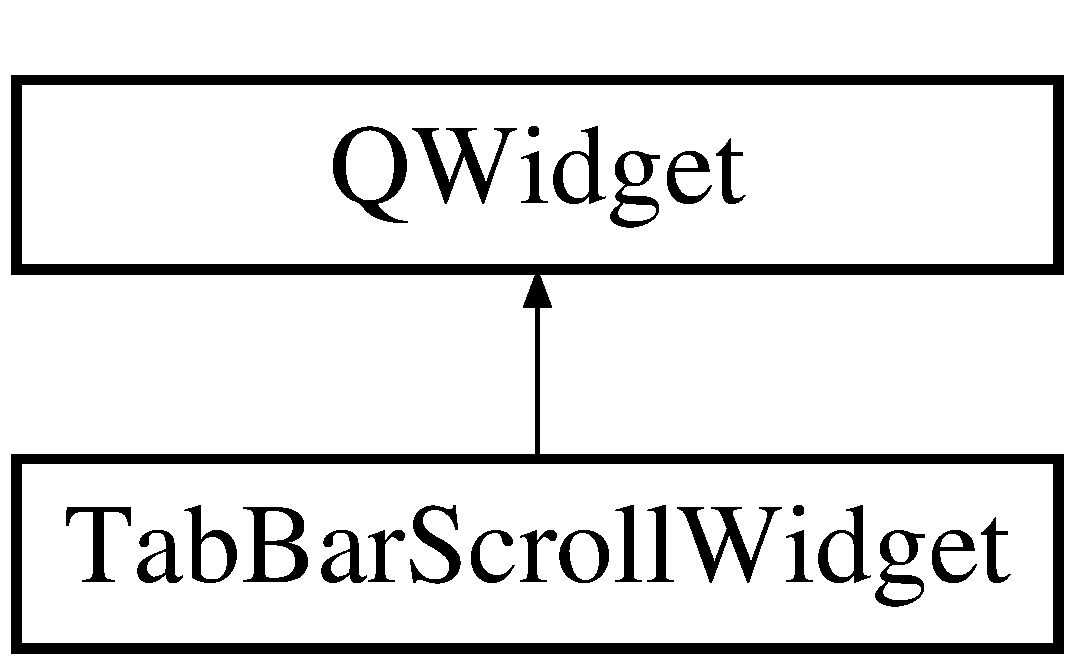
\includegraphics[height=2cm]{class_tab_bar_scroll_widget}
\end{center}
\end{figure}
\subsection*{Public Slots}
\begin{DoxyCompactItemize}
\item 
void \hyperlink{class_tab_bar_scroll_widget_a05bdaea447574f7fb718cd353e98400b}{ensureVisible} (int index=-\/1, int xmargin=132)
\item 
void \hyperlink{class_tab_bar_scroll_widget_a525f4d6a01724eab689c59e35a134789}{scrollToLeft} (int n=5, QEasingCurve::Type type=QEasingCurve::OutQuad)
\item 
void \hyperlink{class_tab_bar_scroll_widget_aae5b0963318e3b84a301df74fcfceb3e}{scrollToRight} (int n=5, QEasingCurve::Type type=QEasingCurve::OutQuad)
\item 
void \hyperlink{class_tab_bar_scroll_widget_aef9cc5e3e46b87fa9a039e62cdadc999}{scrollToLeftEdge} ()
\item 
void \hyperlink{class_tab_bar_scroll_widget_a8c700b63b084d5fec121ff07061763f6}{scrollToRightEdge} ()
\item 
\hypertarget{class_tab_bar_scroll_widget_aa3803469255e43631cc765f42b48f5b8}{
void {\bfseries setUpLayout} ()}
\label{class_tab_bar_scroll_widget_aa3803469255e43631cc765f42b48f5b8}

\end{DoxyCompactItemize}
\subsection*{Public Member Functions}
\begin{DoxyCompactItemize}
\item 
\hypertarget{class_tab_bar_scroll_widget_ac9f5578f01099a3f0b07ffebf79be736}{
{\bfseries TabBarScrollWidget} (\hyperlink{class_q_tab_bar}{QTabBar} $\ast$tabBar, \hyperlink{class_q_widget}{QWidget} $\ast$parent=0)}
\label{class_tab_bar_scroll_widget_ac9f5578f01099a3f0b07ffebf79be736}

\item 
\hypertarget{class_tab_bar_scroll_widget_a8cdb56dbc58327427e8283d563558ab2}{
\hyperlink{class_q_tab_bar}{QTabBar} $\ast$ {\bfseries tabBar} ()}
\label{class_tab_bar_scroll_widget_a8cdb56dbc58327427e8283d563558ab2}

\item 
\hypertarget{class_tab_bar_scroll_widget_af3bb9c0713ded8308611e198f834fda1}{
QScrollArea $\ast$ {\bfseries scrollArea} ()}
\label{class_tab_bar_scroll_widget_af3bb9c0713ded8308611e198f834fda1}

\item 
\hypertarget{class_tab_bar_scroll_widget_a850f2ea062974be7be1f6b58761a8a79}{
\hyperlink{class_tab_scroll_bar}{TabScrollBar} $\ast$ {\bfseries scrollBar} ()}
\label{class_tab_bar_scroll_widget_a850f2ea062974be7be1f6b58761a8a79}

\item 
\hypertarget{class_tab_bar_scroll_widget_a9d361a6291b10a23c1545a8101e562c3}{
void {\bfseries scrollByWheel} (QWheelEvent $\ast$event)}
\label{class_tab_bar_scroll_widget_a9d361a6291b10a23c1545a8101e562c3}

\item 
\hypertarget{class_tab_bar_scroll_widget_ad5154497fc810c2129bcdce8bd0f4725}{
int {\bfseries scrollButtonsWidth} () const }
\label{class_tab_bar_scroll_widget_ad5154497fc810c2129bcdce8bd0f4725}

\item 
\hypertarget{class_tab_bar_scroll_widget_af7bf35a9970590eef45fafb19cb3931f}{
bool {\bfseries usesScrollButtons} () const }
\label{class_tab_bar_scroll_widget_af7bf35a9970590eef45fafb19cb3931f}

\item 
\hypertarget{class_tab_bar_scroll_widget_a0a95792b2d0aad18ac5929afc5197414}{
void {\bfseries setUsesScrollButtons} (bool useButtons)}
\label{class_tab_bar_scroll_widget_a0a95792b2d0aad18ac5929afc5197414}

\item 
\hypertarget{class_tab_bar_scroll_widget_acefc10337736ee7b075e27ad53dd2441}{
bool {\bfseries isOverflowed} () const }
\label{class_tab_bar_scroll_widget_acefc10337736ee7b075e27ad53dd2441}

\item 
\hypertarget{class_tab_bar_scroll_widget_a6ea868a68da8ecf19a970c3a8e8bf8cc}{
int {\bfseries tabAt} (const QPoint \&pos) const }
\label{class_tab_bar_scroll_widget_a6ea868a68da8ecf19a970c3a8e8bf8cc}

\item 
\hypertarget{class_tab_bar_scroll_widget_ae850dc2df1840e30e2bf3220a473419c}{
void {\bfseries enableBluredBackground} (bool enable)}
\label{class_tab_bar_scroll_widget_ae850dc2df1840e30e2bf3220a473419c}

\end{DoxyCompactItemize}
\subsection*{Private Slots}
\begin{DoxyCompactItemize}
\item 
\hypertarget{class_tab_bar_scroll_widget_aa2df438b67f0f1ab1b5720b2fa8e2dc0}{
void {\bfseries overFlowChanged} (bool overflowed)}
\label{class_tab_bar_scroll_widget_aa2df438b67f0f1ab1b5720b2fa8e2dc0}

\item 
void \hyperlink{class_tab_bar_scroll_widget_a05a239bfcf3fe7853b75dd8366132406}{scrollStart} ()
\item 
\hypertarget{class_tab_bar_scroll_widget_a1ad0599b9615485b62f4630c01379ba5}{
void {\bfseries updateScrollButtonsState} ()}
\label{class_tab_bar_scroll_widget_a1ad0599b9615485b62f4630c01379ba5}

\end{DoxyCompactItemize}
\subsection*{Private Member Functions}
\begin{DoxyCompactItemize}
\item 
\hypertarget{class_tab_bar_scroll_widget_a31dce9b238060a7c0355d7d14100cb24}{
void {\bfseries mouseMoveEvent} (QMouseEvent $\ast$event)}
\label{class_tab_bar_scroll_widget_a31dce9b238060a7c0355d7d14100cb24}

\item 
\hypertarget{class_tab_bar_scroll_widget_a02deb9f280753efe681a14d047da4f63}{
void {\bfseries resizeEvent} (QResizeEvent $\ast$event)}
\label{class_tab_bar_scroll_widget_a02deb9f280753efe681a14d047da4f63}

\end{DoxyCompactItemize}
\subsection*{Private Attributes}
\begin{DoxyCompactItemize}
\item 
\hypertarget{class_tab_bar_scroll_widget_a7d2f788208ded4cfa19a8771822a225e}{
\hyperlink{class_q_tab_bar}{QTabBar} $\ast$ {\bfseries m\_\-tabBar}}
\label{class_tab_bar_scroll_widget_a7d2f788208ded4cfa19a8771822a225e}

\item 
\hypertarget{class_tab_bar_scroll_widget_aad4c2d106207378354e296a8aa3b0da9}{
QScrollArea $\ast$ {\bfseries m\_\-scrollArea}}
\label{class_tab_bar_scroll_widget_aad4c2d106207378354e296a8aa3b0da9}

\item 
\hypertarget{class_tab_bar_scroll_widget_a6541eebd7a4b72fa656d721e34d92c8a}{
\hyperlink{class_tab_scroll_bar}{TabScrollBar} $\ast$ {\bfseries m\_\-scrollBar}}
\label{class_tab_bar_scroll_widget_a6541eebd7a4b72fa656d721e34d92c8a}

\item 
\hypertarget{class_tab_bar_scroll_widget_a830c235df1e193a473aa732f0eccc62b}{
ToolButton $\ast$ {\bfseries m\_\-rightScrollButton}}
\label{class_tab_bar_scroll_widget_a830c235df1e193a473aa732f0eccc62b}

\item 
\hypertarget{class_tab_bar_scroll_widget_a9aef94590ad92d0500aac2317a61f22c}{
ToolButton $\ast$ {\bfseries m\_\-leftScrollButton}}
\label{class_tab_bar_scroll_widget_a9aef94590ad92d0500aac2317a61f22c}

\item 
\hypertarget{class_tab_bar_scroll_widget_a04d28c33b65d33b253367838da438707}{
bool {\bfseries m\_\-usesScrollButtons}}
\label{class_tab_bar_scroll_widget_a04d28c33b65d33b253367838da438707}

\item 
\hypertarget{class_tab_bar_scroll_widget_a5e4e96c4df52961d0dc928da8c7f63f7}{
bool {\bfseries m\_\-bluredBackground}}
\label{class_tab_bar_scroll_widget_a5e4e96c4df52961d0dc928da8c7f63f7}

\item 
\hypertarget{class_tab_bar_scroll_widget_a17714d4a6564ba0c61c074f99836cfa8}{
int {\bfseries m\_\-totalDeltas}}
\label{class_tab_bar_scroll_widget_a17714d4a6564ba0c61c074f99836cfa8}

\end{DoxyCompactItemize}


\subsection{Detailed Description}
Adds scrolling feature to \hyperlink{class_q_tab_bar}{QTabBar}. It has a horizontal layout containing: m\_\-leftScrollButton $|$ m\_\-scrollArea $|$ m\_\-rightScrollButton

m\_\-scrollArea is a QScrollArea with a \hyperlink{class_tab_bar_helper}{TabBarHelper} as its widget, and it uses a \hyperlink{class_tab_scroll_bar}{TabScrollBar} as its horizontal scrollbar 

\subsection{Member Function Documentation}
\hypertarget{class_tab_bar_scroll_widget_a05bdaea447574f7fb718cd353e98400b}{
\index{TabBarScrollWidget@{TabBarScrollWidget}!ensureVisible@{ensureVisible}}
\index{ensureVisible@{ensureVisible}!TabBarScrollWidget@{TabBarScrollWidget}}
\subsubsection[{ensureVisible}]{\setlength{\rightskip}{0pt plus 5cm}void TabBarScrollWidget::ensureVisible (int {\em index} = {\ttfamily -\/1}, \/  int {\em xmargin} = {\ttfamily 132})\hspace{0.3cm}{\ttfamily  \mbox{[}slot\mbox{]}}}}
\label{class_tab_bar_scroll_widget_a05bdaea447574f7fb718cd353e98400b}


scrolls to index or currentIndex() if index is -\/1 (default) 

\hypertarget{class_tab_bar_scroll_widget_a05a239bfcf3fe7853b75dd8366132406}{
\index{TabBarScrollWidget@{TabBarScrollWidget}!scrollStart@{scrollStart}}
\index{scrollStart@{scrollStart}!TabBarScrollWidget@{TabBarScrollWidget}}
\subsubsection[{scrollStart}]{\setlength{\rightskip}{0pt plus 5cm}void TabBarScrollWidget::scrollStart ()\hspace{0.3cm}{\ttfamily  \mbox{[}private, slot\mbox{]}}}}
\label{class_tab_bar_scroll_widget_a05a239bfcf3fe7853b75dd8366132406}


used for non-\/stop linear scrolling when mouse is pressed on scroll buttons 

\hypertarget{class_tab_bar_scroll_widget_a525f4d6a01724eab689c59e35a134789}{
\index{TabBarScrollWidget@{TabBarScrollWidget}!scrollToLeft@{scrollToLeft}}
\index{scrollToLeft@{scrollToLeft}!TabBarScrollWidget@{TabBarScrollWidget}}
\subsubsection[{scrollToLeft}]{\setlength{\rightskip}{0pt plus 5cm}void TabBarScrollWidget::scrollToLeft (int {\em n} = {\ttfamily 5}, \/  QEasingCurve::Type {\em type} = {\ttfamily QEasingCurve::OutQuad})\hspace{0.3cm}{\ttfamily  \mbox{[}slot\mbox{]}}}}
\label{class_tab_bar_scroll_widget_a525f4d6a01724eab689c59e35a134789}


scrolls to smaller values by n singleStep() 

\hypertarget{class_tab_bar_scroll_widget_aef9cc5e3e46b87fa9a039e62cdadc999}{
\index{TabBarScrollWidget@{TabBarScrollWidget}!scrollToLeftEdge@{scrollToLeftEdge}}
\index{scrollToLeftEdge@{scrollToLeftEdge}!TabBarScrollWidget@{TabBarScrollWidget}}
\subsubsection[{scrollToLeftEdge}]{\setlength{\rightskip}{0pt plus 5cm}void TabBarScrollWidget::scrollToLeftEdge ()\hspace{0.3cm}{\ttfamily  \mbox{[}slot\mbox{]}}}}
\label{class_tab_bar_scroll_widget_aef9cc5e3e46b87fa9a039e62cdadc999}


scrolls to minimum using QEasingCurve::OutQuad 

\hypertarget{class_tab_bar_scroll_widget_aae5b0963318e3b84a301df74fcfceb3e}{
\index{TabBarScrollWidget@{TabBarScrollWidget}!scrollToRight@{scrollToRight}}
\index{scrollToRight@{scrollToRight}!TabBarScrollWidget@{TabBarScrollWidget}}
\subsubsection[{scrollToRight}]{\setlength{\rightskip}{0pt plus 5cm}void TabBarScrollWidget::scrollToRight (int {\em n} = {\ttfamily 5}, \/  QEasingCurve::Type {\em type} = {\ttfamily QEasingCurve::OutQuad})\hspace{0.3cm}{\ttfamily  \mbox{[}slot\mbox{]}}}}
\label{class_tab_bar_scroll_widget_aae5b0963318e3b84a301df74fcfceb3e}


scrolls to bigger values by n singleStep() 

\hypertarget{class_tab_bar_scroll_widget_a8c700b63b084d5fec121ff07061763f6}{
\index{TabBarScrollWidget@{TabBarScrollWidget}!scrollToRightEdge@{scrollToRightEdge}}
\index{scrollToRightEdge@{scrollToRightEdge}!TabBarScrollWidget@{TabBarScrollWidget}}
\subsubsection[{scrollToRightEdge}]{\setlength{\rightskip}{0pt plus 5cm}void TabBarScrollWidget::scrollToRightEdge ()\hspace{0.3cm}{\ttfamily  \mbox{[}slot\mbox{]}}}}
\label{class_tab_bar_scroll_widget_a8c700b63b084d5fec121ff07061763f6}


scrolls to maximum using QEasingCurve::OutQuad 



The documentation for this class was generated from the following file:\begin{DoxyCompactItemize}
\item 
E:/Programming/QupZilla-\/Project/qupzilla/src/lib/tabwidget/combotabbar.h\end{DoxyCompactItemize}

\hypertarget{class_tab_scroll_bar}{
\section{TabScrollBar Class Reference}
\label{class_tab_scroll_bar}\index{TabScrollBar@{TabScrollBar}}
}
Inheritance diagram for TabScrollBar:\begin{figure}[H]
\begin{center}
\leavevmode
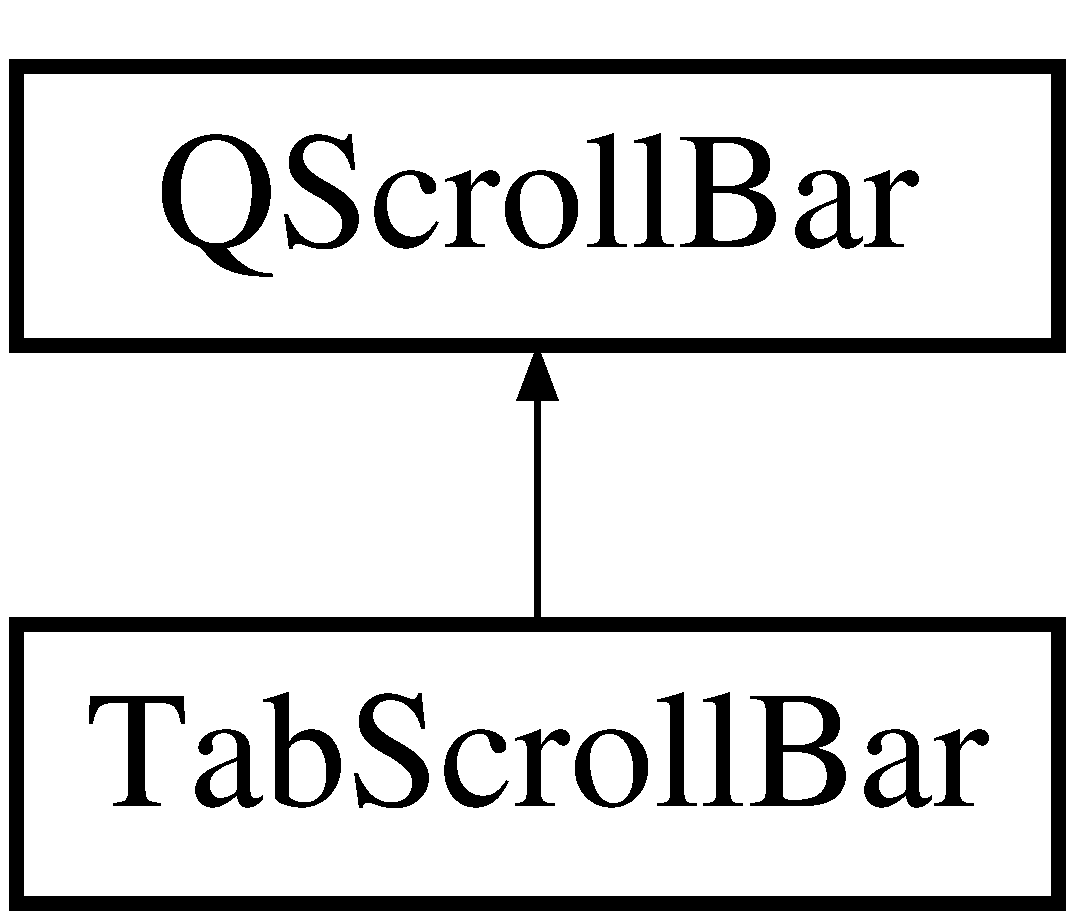
\includegraphics[height=2cm]{class_tab_scroll_bar}
\end{center}
\end{figure}
\subsection*{Public Member Functions}
\begin{DoxyCompactItemize}
\item 
\hypertarget{class_tab_scroll_bar_ad3f68bba5a829dff8801bb7c00631cae}{
{\bfseries TabScrollBar} (\hyperlink{class_q_widget}{QWidget} $\ast$parent=0)}
\label{class_tab_scroll_bar_ad3f68bba5a829dff8801bb7c00631cae}

\item 
\hypertarget{class_tab_scroll_bar_a0c7cc84d20a2f815a1e72c7c5c36884c}{
void {\bfseries animateToValue} (int to, QEasingCurve::Type type=QEasingCurve::OutQuad)}
\label{class_tab_scroll_bar_a0c7cc84d20a2f815a1e72c7c5c36884c}

\end{DoxyCompactItemize}
\subsection*{Private Attributes}
\begin{DoxyCompactItemize}
\item 
\hypertarget{class_tab_scroll_bar_aaf92339a1a9d6cb3a206c8d07819cae0}{
QPropertyAnimation $\ast$ {\bfseries m\_\-animation}}
\label{class_tab_scroll_bar_aaf92339a1a9d6cb3a206c8d07819cae0}

\end{DoxyCompactItemize}


The documentation for this class was generated from the following file:\begin{DoxyCompactItemize}
\item 
E:/Programming/QupZilla-\/Project/qupzilla/src/lib/tabwidget/combotabbar.h\end{DoxyCompactItemize}

\hypertarget{class_tab_stacked_widget}{
\section{TabStackedWidget Class Reference}
\label{class_tab_stacked_widget}\index{TabStackedWidget@{TabStackedWidget}}
}
Inheritance diagram for TabStackedWidget:\begin{figure}[H]
\begin{center}
\leavevmode
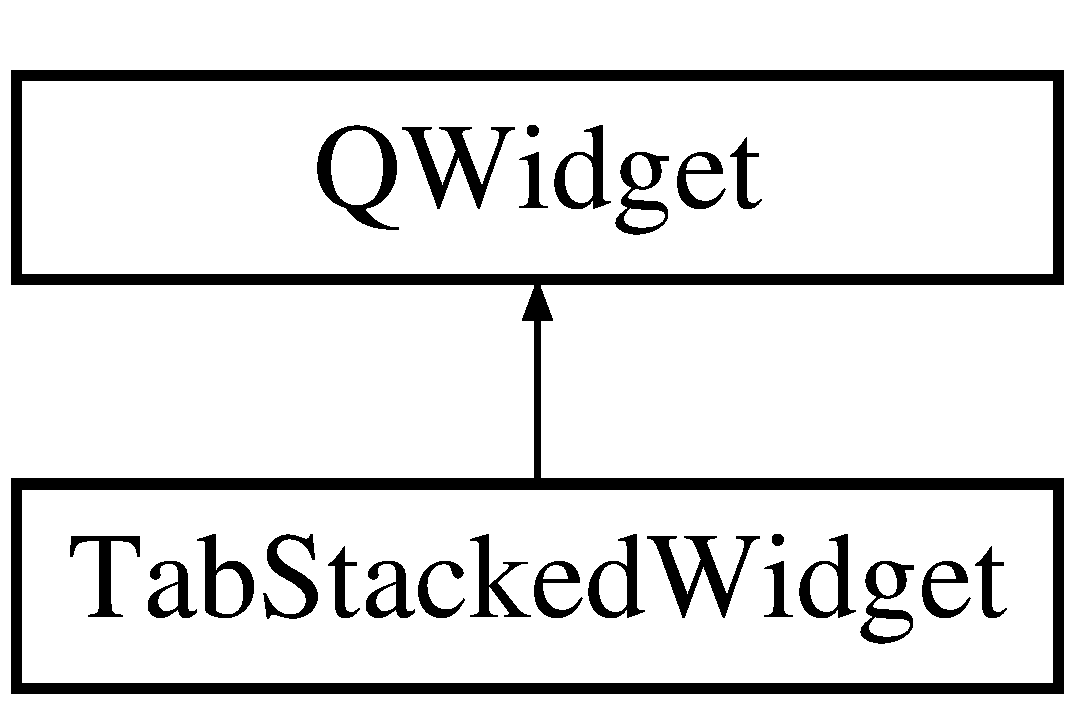
\includegraphics[height=2cm]{class_tab_stacked_widget}
\end{center}
\end{figure}
\subsection*{Public Slots}
\begin{DoxyCompactItemize}
\item 
\hypertarget{class_tab_stacked_widget_a74183fe7bd0f0ff5fcc57ba1435236cc}{
void {\bfseries setCurrentIndex} (int index)}
\label{class_tab_stacked_widget_a74183fe7bd0f0ff5fcc57ba1435236cc}

\item 
\hypertarget{class_tab_stacked_widget_ae8779463e03448a6336006e23944a534}{
void {\bfseries setCurrentWidget} (\hyperlink{class_q_widget}{QWidget} $\ast$widget)}
\label{class_tab_stacked_widget_ae8779463e03448a6336006e23944a534}

\item 
\hypertarget{class_tab_stacked_widget_a3b3cba2736761f0ef10ef15e50904f33}{
void {\bfseries setUpLayout} ()}
\label{class_tab_stacked_widget_a3b3cba2736761f0ef10ef15e50904f33}

\end{DoxyCompactItemize}
\subsection*{Signals}
\begin{DoxyCompactItemize}
\item 
\hypertarget{class_tab_stacked_widget_a9378f9c896957d9bb37bc6fdc180981c}{
void {\bfseries currentChanged} (int index)}
\label{class_tab_stacked_widget_a9378f9c896957d9bb37bc6fdc180981c}

\item 
\hypertarget{class_tab_stacked_widget_af615c93acb887e3291a705935b87fb86}{
void {\bfseries tabCloseRequested} (int index)}
\label{class_tab_stacked_widget_af615c93acb887e3291a705935b87fb86}

\end{DoxyCompactItemize}
\subsection*{Public Member Functions}
\begin{DoxyCompactItemize}
\item 
\hypertarget{class_tab_stacked_widget_af74e31a77c3b4fc04a8444ac3c8a2f14}{
{\bfseries TabStackedWidget} (\hyperlink{class_q_widget}{QWidget} $\ast$parent=0)}
\label{class_tab_stacked_widget_af74e31a77c3b4fc04a8444ac3c8a2f14}

\item 
\hypertarget{class_tab_stacked_widget_a354c44a4559ef1c7d40672cd7de5c45c}{
\hyperlink{class_combo_tab_bar}{ComboTabBar} $\ast$ {\bfseries tabBar} ()}
\label{class_tab_stacked_widget_a354c44a4559ef1c7d40672cd7de5c45c}

\item 
\hypertarget{class_tab_stacked_widget_a61e38c15cd94e9a26c2fbfaea33f1f68}{
void {\bfseries setTabBar} (\hyperlink{class_combo_tab_bar}{ComboTabBar} $\ast$tb)}
\label{class_tab_stacked_widget_a61e38c15cd94e9a26c2fbfaea33f1f68}

\item 
\hypertarget{class_tab_stacked_widget_a16e2efde830506e8d5d7e4c7cc051d38}{
bool {\bfseries documentMode} () const }
\label{class_tab_stacked_widget_a16e2efde830506e8d5d7e4c7cc051d38}

\item 
\hypertarget{class_tab_stacked_widget_a5664687a2ebd33508410362764f587a3}{
void {\bfseries setDocumentMode} (bool enabled)}
\label{class_tab_stacked_widget_a5664687a2ebd33508410362764f587a3}

\item 
\hypertarget{class_tab_stacked_widget_a763e40673682bdfaebd518008a58f1a1}{
int {\bfseries addTab} (\hyperlink{class_q_widget}{QWidget} $\ast$widget, const QString \&label, bool pinned=false)}
\label{class_tab_stacked_widget_a763e40673682bdfaebd518008a58f1a1}

\item 
\hypertarget{class_tab_stacked_widget_ab2a2466ef7ae88f9813f473e6452bd00}{
int {\bfseries insertTab} (int index, \hyperlink{class_q_widget}{QWidget} $\ast$widget, const QString \&label, bool pinned=false)}
\label{class_tab_stacked_widget_ab2a2466ef7ae88f9813f473e6452bd00}

\item 
\hypertarget{class_tab_stacked_widget_a72e1cf12a94bba3216b318efa39d0b09}{
QString {\bfseries tabText} (int index) const }
\label{class_tab_stacked_widget_a72e1cf12a94bba3216b318efa39d0b09}

\item 
\hypertarget{class_tab_stacked_widget_a9eb31d54313fadd7240438f98206343f}{
void {\bfseries setTabText} (int index, const QString \&label)}
\label{class_tab_stacked_widget_a9eb31d54313fadd7240438f98206343f}

\item 
\hypertarget{class_tab_stacked_widget_a38c74726adf08931c0035f5232d993b2}{
QString {\bfseries tabToolTip} (int index) const }
\label{class_tab_stacked_widget_a38c74726adf08931c0035f5232d993b2}

\item 
\hypertarget{class_tab_stacked_widget_a695722b14055d2cf2db50cc1ac44796c}{
void {\bfseries setTabToolTip} (int index, const QString \&tip)}
\label{class_tab_stacked_widget_a695722b14055d2cf2db50cc1ac44796c}

\item 
\hypertarget{class_tab_stacked_widget_a189fe7535ae814fdf43ba1abff94678c}{
int {\bfseries pinUnPinTab} (int index, const QString \&title=QString())}
\label{class_tab_stacked_widget_a189fe7535ae814fdf43ba1abff94678c}

\item 
\hypertarget{class_tab_stacked_widget_a3c2ace9ea78144c9fbbce3bf0a299e89}{
void {\bfseries removeTab} (int index)}
\label{class_tab_stacked_widget_a3c2ace9ea78144c9fbbce3bf0a299e89}

\item 
\hypertarget{class_tab_stacked_widget_ab9b45fb1c0872f2f674a8f1d4c00c945}{
int {\bfseries currentIndex} () const }
\label{class_tab_stacked_widget_ab9b45fb1c0872f2f674a8f1d4c00c945}

\item 
\hypertarget{class_tab_stacked_widget_ab630369d144ed5bf9df432dba8a49e3d}{
\hyperlink{class_q_widget}{QWidget} $\ast$ {\bfseries currentWidget} () const }
\label{class_tab_stacked_widget_ab630369d144ed5bf9df432dba8a49e3d}

\item 
\hypertarget{class_tab_stacked_widget_ae178d95c603dec72c09f49ed2ed39761}{
\hyperlink{class_q_widget}{QWidget} $\ast$ {\bfseries widget} (int index) const }
\label{class_tab_stacked_widget_ae178d95c603dec72c09f49ed2ed39761}

\item 
\hypertarget{class_tab_stacked_widget_ae67cadc2b20fbfd520305ba57d3d1f32}{
int {\bfseries indexOf} (\hyperlink{class_q_widget}{QWidget} $\ast$widget) const }
\label{class_tab_stacked_widget_ae67cadc2b20fbfd520305ba57d3d1f32}

\item 
\hypertarget{class_tab_stacked_widget_a235c2b586a7f8ab231acf2e0472ce3ae}{
int {\bfseries count} () const }
\label{class_tab_stacked_widget_a235c2b586a7f8ab231acf2e0472ce3ae}

\end{DoxyCompactItemize}
\subsection*{Protected Member Functions}
\begin{DoxyCompactItemize}
\item 
\hypertarget{class_tab_stacked_widget_a54c4e17b00913256973d890554fab03d}{
bool {\bfseries eventFilter} (QObject $\ast$obj, QEvent $\ast$event)}
\label{class_tab_stacked_widget_a54c4e17b00913256973d890554fab03d}

\item 
\hypertarget{class_tab_stacked_widget_a2ee5e5a190b7c294ecf72e7a75091df8}{
void {\bfseries keyPressEvent} (QKeyEvent $\ast$event)}
\label{class_tab_stacked_widget_a2ee5e5a190b7c294ecf72e7a75091df8}

\end{DoxyCompactItemize}
\subsection*{Private Slots}
\begin{DoxyCompactItemize}
\item 
\hypertarget{class_tab_stacked_widget_a6b1760758e58f1e28762ab1f8bac5eef}{
void {\bfseries showTab} (int index)}
\label{class_tab_stacked_widget_a6b1760758e58f1e28762ab1f8bac5eef}

\item 
\hypertarget{class_tab_stacked_widget_a21355edb24806d536d066b53405af0dc}{
void {\bfseries tabWasMoved} (int from, int to)}
\label{class_tab_stacked_widget_a21355edb24806d536d066b53405af0dc}

\item 
\hypertarget{class_tab_stacked_widget_afb87ed29ff819b1bd3ecea878249a97c}{
void {\bfseries tabWasRemoved} (int index)}
\label{class_tab_stacked_widget_afb87ed29ff819b1bd3ecea878249a97c}

\end{DoxyCompactItemize}
\subsection*{Private Member Functions}
\begin{DoxyCompactItemize}
\item 
\hypertarget{class_tab_stacked_widget_a93ea6c0c29cfe0fa58366726e97a5da2}{
bool {\bfseries validIndex} (int index) const }
\label{class_tab_stacked_widget_a93ea6c0c29cfe0fa58366726e97a5da2}

\end{DoxyCompactItemize}
\subsection*{Private Attributes}
\begin{DoxyCompactItemize}
\item 
\hypertarget{class_tab_stacked_widget_a4f7c1e2a129fe25475330ce31a543e20}{
QStackedWidget $\ast$ {\bfseries m\_\-stack}}
\label{class_tab_stacked_widget_a4f7c1e2a129fe25475330ce31a543e20}

\item 
\hypertarget{class_tab_stacked_widget_a70ba27bb0c4b3499eb6484f4e1532fde}{
\hyperlink{class_combo_tab_bar}{ComboTabBar} $\ast$ {\bfseries m\_\-tabBar}}
\label{class_tab_stacked_widget_a70ba27bb0c4b3499eb6484f4e1532fde}

\item 
\hypertarget{class_tab_stacked_widget_a11003c41b44f06a5248939be3a2ed5f1}{
QVBoxLayout $\ast$ {\bfseries m\_\-mainLayout}}
\label{class_tab_stacked_widget_a11003c41b44f06a5248939be3a2ed5f1}

\item 
\hypertarget{class_tab_stacked_widget_a502d1a8effcefef8a899ed85f945e60b}{
bool {\bfseries m\_\-dirtyTabBar}}
\label{class_tab_stacked_widget_a502d1a8effcefef8a899ed85f945e60b}

\end{DoxyCompactItemize}


The documentation for this class was generated from the following file:\begin{DoxyCompactItemize}
\item 
E:/Programming/QupZilla-\/Project/qupzilla/src/lib/tabwidget/tabstackedwidget.h\end{DoxyCompactItemize}

\printindex
\end{document}
